\section{Introduction}

The Integrity and Authenticity (I\&A) work package is concerned with
supporting longevity of workflows; i.e.~that workflows created today
continue to be usable and useful in years to come. It emphasises
proactive detection and prevention of undesired degradation in
performance.

This evaluation assesses the performance of two main tools created to
proactively evaluate and monitor the health of Research Objects, and in
particular those containing workfows. The focus of our work has been
informed by an analysis of the causes of workflow decay
\cite{Zhao-2012}, which highlighted the role of researchers in
maintaining and adapting workflows to survive in a changing environment,
and the importance of supporting documentation for human consumption as
well as computational tools for analysis and preservation - that is, we
need to treat this as an exercise in \emph{conservation} of function
rather than merely \emph{preservation} of bits.

This distinction between conservation and preservation is perhaps best
illustrated by studies of biological species and ecosystems. Historical
study of species was primarily concerned with collecting and preserving
specimens in museums. Current activities also focus on conservation:
understanding the dynamics of interaction between species and their
environment, and making selected interventions that help species to
survive as living creatures. And so it is with workflows: their utility
stems from their dynamic behaviour as executing processes, interacting
with external datasets and services to produce scientifically useful
results.

For example, one set of pre-existing bioinformatic workflows we studied
(\emph{Analysis of KEGG workflows decay}\footnote{\url{http://www.wf4ever-project.org/wiki/display/docs/Showcase+100.+Analysis+of+KEGG+workflows+decay}})
made use of genetic pathway information from services provided by
\emph{Kyoto Encyclopedia of Genes and Genomes (KEGG)}\footnote{\url{http://www.genome.jp/kegg/}}.
In 2012, KEGG announced that they were upgrading their service to use a
new REST interface, and discontinuing the previously offered Web Service
offerings. Clearly, preserved workflows that use these services would
cease to function as designed, and would need to be updated to use the
new services offered if they were to continue to be runnable. This kind
of intervention is what we would describe as a ``conservation'' action,
be it applied manually or automatically. Part of our focus in this work
has been to detect the need for such intervention, a clearly needed
first step to applying it by any means. Separate and ongoing research
\cite{Garijo-2012} is concerned with automatic characterization and
eventual application of a required intervention, but such work is not
covered here.

Until such time as all conservation actions can be automatically
determined and applied, we also need to support researchers who are
faced with decayed workflows. Our project colleagues have analyzed their
workflow-based research activities and come up with a set of
requirements\footnote{\url{http://wf4ever.github.io/Requirements/docs/output/UserRequirements-all.html}}
and best practices in workflow design \cite{Kettne-2012}, which are
aimed at providing such support. Another part of our focus has been to
analyze Workflow-centric Research Objects to report on the extent to
which such practices have been followed (e.g., checking that the
description of a workflow's intended purpose and a design sketch have
been provided).

The tools we have developed within the Wf4Ever project to support these
goals are:

\begin{itemize}
\itemsep1pt\parskip0pt\parsep0pt
\item
  a checklist evaluation service, used to provide a point-in-time
  evaluation of the status of a Research Object with respect to decay
  detection and its conformance to community best practices.
\item
  a stability evaluation service, which builds upon the checklist
  service to provide a view of how the Research Object, considered as a
  evolving entity in a dynamic environment, continues to maintain these
  qualities over time.
\end{itemize}

These evaluation services are designed to guide researchers to provide
sufficient supporting information to allow future researchers to perform
any conservation interventions that may be needed (is it good enough?),
to provide alerting information when interventions are needed (something
has broken), and to provide some indication whether conservation is a
viable option for a given workflow (is it suitable for reuse?).

As anticipated in the project proposal, provenance is a thread that runs
through many of the I\&A assessments. Provenance is not an end in
itself, but is used in the evaluation of features that have been
identified as useful for workflow conservation (e.g.~does a workflow
have example inputs and outputs that can be used to verify its correct
operation?). As such, the evaluations that follow don't specifically
mention provenance, but evaluation some of the identified requirements
does depend on availability of provenance information. Much of our work
on provenance has been in the form of contributions to the W3C
Provenance Working Group\footnote{\url{http://www.w3.org/2011/prov/wiki/Main_Page}},
and as such has been validated through the normal processes of open
standards review and adoption: acceptance as a full W3C Recommendation
entails community consensus and successful adoption of the provenance
model and ontology.

\section{Evaluation framework}

Our evaluation of the I\&A tools is structured around the guidelines
provided by the UK's Software Sustainability Institute (SSI): Software
evaluation guide \cite{SSI-guide}, Software Evaluation: Tutorial-based
Assessment \cite{SSI-tutorial} and Software Evaluation: Criteria-based
Assessment \cite{SSI-criteria}.

The SSI evaluation guides target three kinds of user: end-users (i.e.,
non-developers who will employ the software), developer-users (i.e.,
developers who will use APIs and other middleware facilities provided in
the creation of some wider application) and developers (i.e., those
tasked with enhancing or repairing the software).

The SSI guides further describe two software evaluation approaches.
Tutorial-based assessment is based on specific tasks to be accomplished
by a user, who reports on the experience running those tasks, and
Criteria-based assessment on a number or criteria which may be checked
depending on the quality and status of the software. There is a fair
degree of overlap between the two evaluation approaches in the topics
that they are intended to cover, which we have tried to minmimize in the
adaptation of the SSI topic coverage reported here.

For user-facing software components, usability should be described. The
WP4 components are mostly middleware fronted by other parts of the
system (such as myExperiment, RO Portal, etc.), and as such are not
involved in the same level of direct user-facing deployment as those
other components. The main focus of our usability evaluation is
therefore on the developer-user aspects, and the ease and effectiveness
of integration of our components with other parts of the Wf4Ever
reference implementation.

For developers, usability focuses on the ease of accessing, building,
understanding, enhancing and testing the code. There is a strong
connection between developer usability and overall sustainability and
maintainability of a software product, reflected by some overlap in the
topics assessed.

A third dimension to be included in the evaluation is some benchmarking
of the components in order to assess indicators of functional capability
and performance.

Finally, features of the software base and its management structure are
surveyed to get a sense of its sustainability and maintainability, and
what further activities might be needed to make the software into a
fully fledged, sustainable product. Many of the features covered here
relate to the creation and sustenance of a community of users and
developers for the product.

This framework is reflected in the structure of the sections that
follow, which deal with evaluation of the checklist service and
stability service respectively. The overall evaluation reporting
structure for each is as follows:

\begin{enumerate}
\def\labelenumi{\arabic{enumi}.}
\item
  Component description, sufficient to place the evaluation within the
  overall context of the Wf4Ever reference architecture.
\item
  Usability study, reporting on applicable usability and effectiveness
  of the component from:

  \begin{itemize}
  \itemsep1pt\parskip0pt\parsep0pt
  \item
    end-user (researcher) perspective
  \item
    developer-user and system integration perspective
  \item
    developer perspective, for enhancing and repairing the software
  \end{itemize}

  The reporting is based on considerations covered by the SSI
  Tutorial-based Assessment \cite{SSI-tutorial}, adapted to draw upon
  our ongoing evaluation efforts, reflecting the agile nature of our
  development. The survey sub-sections draw particularly from the SSI
  guide.
\item
  Benchmarking: an assessment of functional and performance
  characteristics of the software with respect to the tasks it is
  expected to perform.
\item
  Sustainability and maintainability study, based on the SSI
  Criteria-based Assessment \cite{SSI-criteria}.
\end{enumerate}

\section{Checklist service}

The checklist service, and the associated \emph{Minim} model used to
define checklists, is part of the \emph{RO Manager} software package.
This package contains a collection of tools for creating Research
Objects (ROs) in a local file system, for transferring ROs to and from
the Research Object Digital Library (RODL) component, and for retrieving
and analyzing the content of ROs which are accessed from either the
local file system, or from the Web using a subset of the Research Object
API (ROAPI).

The main part of the RO Manager package is a command line tool that can
perform all of these functions, including checklist evaluation. Also in
the package is a web service, \texttt{ROWeb}, that implements an API for
use by web clients to invoke checklist evaluation of any web-accessible
Research Object. This service is a key element of the Integrity and
Authenticity services implemented by the Wf4Ever project, and is the
main subject of the evaluation in this section.

Also part of the RO Manager package is a facility to present arbitrary
linked data on the web as an ``Overlay RO'' - that is a RO that is a
lightweight overlay on the web of linked data rather than a collection
of resources and links in a repository.

See also:

\begin{itemize}
\itemsep1pt\parskip0pt\parsep0pt
\item
  Wf4Ever: Design, implementation and deployment of Workflow Integrity
  and Authenticity Maintenance components - Phase II \cite{D4.2v2}
\item
  RO-Manager: A Tool for Creating and Manipulating Research Objects to
  Support Reproducibility and Reuse in Sciences \cite{ro_manager}.
\item
  A Checklist-Based Approach for Quality Assessment of Scientific
  Information \cite{ro_checklist}.
\item
  RO decay detection using checklists\footnote{\url{http://www.wf4ever-project.org/wiki/display/docs/RO+decay+detection+using+checklists}}
\item
  RO checklist evaluation API\footnote{\url{http://www.wf4ever-project.org/wiki/display/docs/RO+checklist+evaluation+API}}
\item
  Checklist traffic light API\footnote{\url{http://www.wf4ever-project.org/wiki/display/docs/Checklist+traffic+light+API}}
\end{itemize}

\subsection{Component description}

The checklist service takes an RO, a Minim checklist description and
other parameters, and on the basis of these performs an evaluation of
the RO or specified resource and returns a result indicating how well
the requirements of the checklist were satisfied.

The checklist that forms the basis of the analysis is itself described
by an RDF resource on the web, using our ``Minim'' model. Using on this
checklist description, the checklist service can perform an open-ended
range of quality evaluations, which may depend on the nature of the
target resource or RO, and the purpose for which it is evaluated. The
checklist description and supporting software is designed to be
extensible to allow new quality requirements to be introduced as they
may be needed. The checklist model is described in D4.2v2 \cite{D4.2v2}
and in a paper presented at the Third Linked Science Workshop
\cite{ro_checklist}.

\subsection{Usability}

The usability survey references these project resources:

\begin{itemize}
\itemsep1pt\parskip0pt\parsep0pt
\item
  Checklist service README file\footnote{\url{https://github.com/wf4ever/ro-manager/blob/master/src/roweb/README.md}
    (README file for checklist service software)}
\item
  RO Manager project in Github\footnote{\url{https://github.com/wf4ever/ro-manager}}
\item
  RO Manager software distribution at PyPI\footnote{\url{https://pypi.python.org/pypi/ro-manager}}
\item
  RO Manager FAQ\footnote{\url{http://www.wf4ever-project.org/wiki/display/docs/RO+Manager+FAQ}}
\item
  Wf4Ever sandbox configuration information\footnote{\url{http://www.wf4ever-project.org/wiki/display/docs/Sandbox+configuration}}
\end{itemize}

\subsubsection{User perspective}

This component is not used directly by an end user. Rather, it is called
by other user-facing Wf4Ever components to provide information about how
well RO meets some designated criteria. As such, it has not been
subjected to a separate usability study.

User presentation of checklist results is handled by the RO Portal
\cite{D1.2v4} (section 4.1), and by the checklist trafic-light service
\cite{D1.2v4} (section 4.3). The RO-enabled myExperiment\footnote{\url{http://alpha2.myexperiment.org/}}
uses the traffic light service to construct a progress bar and pop-up
traffic-light displays \cite{D1.2v4} (section 4.3).

\textbf{Survey}

\textbf{General usability:}

The checklist service is not directly viewed by end-users, so this part
of the SSI survey is not applicable.

\textbf{Release packaging:}

\begin{itemize}
\itemsep1pt\parskip0pt\parsep0pt
\item
  Are the binary releases packaged for immediate use in a suitable
  archive format?

  \begin{itemize}
  \itemsep1pt\parskip0pt\parsep0pt
  \item
    Yes: installation via PyPI \footnote{\url{https://pypi.python.org/pypi/ro-manager}}
  \item
    See also the README file
  \end{itemize}
\item
  Is it clear how to get the software from the web site? Does it have
  version numbers?

  \begin{itemize}
  \itemsep1pt\parskip0pt\parsep0pt
  \item
    Yes
  \end{itemize}
\item
  Is it clear from the web site or user doc what other packages are
  required?

  \begin{itemize}
  \itemsep1pt\parskip0pt\parsep0pt
  \item
    Yes
  \end{itemize}
\item
  Is it clear what the licencing and copyright is on the web site?

  \begin{itemize}
  \itemsep1pt\parskip0pt\parsep0pt
  \item
    Yes
  \end{itemize}
\item
  How to get started. Is there a README, FAQ?

  \begin{itemize}
  \itemsep1pt\parskip0pt\parsep0pt
  \item
    Yes
  \end{itemize}
\end{itemize}

\textbf{User documentation:}

\begin{itemize}
\itemsep1pt\parskip0pt\parsep0pt
\item
  Are there relevant user documents?

  \begin{itemize}
  \itemsep1pt\parskip0pt\parsep0pt
  \item
    Yes. See the README file and linked documents.
  \end{itemize}
\item
  Is the user documentation accurate?

  \begin{itemize}
  \itemsep1pt\parskip0pt\parsep0pt
  \item
    It is beleived to be
  \end{itemize}
\item
  Does it partition user, user-developer and developer information or
  mix it all together?

  \begin{itemize}
  \itemsep1pt\parskip0pt\parsep0pt
  \item
    Some partitioning, but not rigorous
  \end{itemize}
\item
  Is the user doc online?

  \begin{itemize}
  \itemsep1pt\parskip0pt\parsep0pt
  \item
    Yes (github and Wf4Ever wiki)
  \end{itemize}
\item
  Are there any supporting tutorials?

  \begin{itemize}
  \itemsep1pt\parskip0pt\parsep0pt
  \item
    No
  \end{itemize}
\item
  Do these list the versions they apply to?

  \begin{itemize}
  \itemsep1pt\parskip0pt\parsep0pt
  \item
    N/A
  \end{itemize}
\item
  Is it task-oriented, structured around helping users achieve their
  tasks?

  \begin{itemize}
  \itemsep1pt\parskip0pt\parsep0pt
  \item
    N/A
  \end{itemize}
\end{itemize}

\textbf{Help and support:}

\begin{itemize}
\itemsep1pt\parskip0pt\parsep0pt
\item
  Is there a list of known bugs and issues, or a bug/issue tracker?

  \begin{itemize}
  \itemsep1pt\parskip0pt\parsep0pt
  \item
    Informally: \url{https://github.com/wf4ever/ro-manager/issues},
    \url{https://github.com/wf4ever/ro-manager/blob/master/TODO.txt}
  \end{itemize}
\item
  Is it clear how to ask for help e.g.~where to e-mail or how to enter
  bugs/issues

  \begin{itemize}
  \itemsep1pt\parskip0pt\parsep0pt
  \item
    No.
  \end{itemize}
\item
  Are there e-mail list archives or forums?

  \begin{itemize}
  \itemsep1pt\parskip0pt\parsep0pt
  \item
    No
  \end{itemize}
\item
  If so, is there evidence of use?

  \begin{itemize}
  \itemsep1pt\parskip0pt\parsep0pt
  \item
    N/A
  \end{itemize}
\item
  Are they searchable?

  \begin{itemize}
  \itemsep1pt\parskip0pt\parsep0pt
  \item
    N/A
  \end{itemize}
\item
  Is there a bug/issue tracker?

  \begin{itemize}
  \itemsep1pt\parskip0pt\parsep0pt
  \item
    Yes (but not much used).
  \item
    \url{https://github.com/wf4ever/ro-manager/issues}
  \item
    \url{https://github.com/wf4ever/ro-manager/blob/master/TODO.txt}
  \item
    \url{https://jira.man.poznan.pl/jira/issues} (not public)
  \end{itemize}
\item
  If so, there evidence of use?

  \begin{itemize}
  \itemsep1pt\parskip0pt\parsep0pt
  \item
    Some, but not consistent
  \end{itemize}
\item
  Does it seem that bugs and issues are resolved or, at least, looked
  at?

  \begin{itemize}
  \itemsep1pt\parskip0pt\parsep0pt
  \item
    Some
  \end{itemize}
\item
  Is it clear what quality of service a user expect in terms of support
  e.g.~best effort, reasonable effort, reply in 24 hours etc.?

  \begin{itemize}
  \itemsep1pt\parskip0pt\parsep0pt
  \item
    No
  \end{itemize}
\item
  Is it clear how to contribute bugs, issues, corrections (e.g.~in
  tutorials or user doc) or ideas?

  \begin{itemize}
  \itemsep1pt\parskip0pt\parsep0pt
  \item
    No, but use of Github offers a generic route.
  \end{itemize}
\end{itemize}

\subsubsection{User-developer perspective}

The checklist provides a simple REST API\footnote{\{http://www.wf4ever-project.org/wiki/display/docs/RO+checklist+evaluation+API\}}
which is used by other component developers to perform a required
evaluation. There is also a ``traffic light API''\footnote{\url{http://www.wf4ever-project.org/wiki/display/docs/Checklist+traffic+light+API}}
that is very similar in style. The REST API has proved quite easy to
use, and has been successfully integrated with minimal additional
guidance from the checklist service developer by other components of the
Wf4Ever project:

\begin{enumerate}
\def\labelenumi{\arabic{enumi}.}
\itemsep1pt\parskip0pt\parsep0pt
\item
  Showcase 47\footnote{\url{http://www.wf4ever-project.org/wiki/pages/viewpage.action?pageId=3506198}}:
  in this activity, the checklist service (developed by Oxford) was
  accessed by an early prototype quality display service (developed
  separately by iSOCO). This was out first attempt to integrate
  Integrity and Authenticity components developed by different project
  members, and showed that the REST style adopted could facilitate
  integration of software components.
\item
  myExperiment\footnote{\url{http://alpha2.myexperiment.org}}: the
  checklist display has been integrated into the display of a
  myExperiment PACK.
\item
  RO Portal\footnote{\{http://sandbox.wf4ever-project.org/portal/\}}:
  the checklist display has been integrated into the RO portal display
  of a Research Object.
\end{enumerate}

To perform a checklist evaluation, a checklist description conforming to
the Minim model\footnote{\url{https://github.com/wf4ever/ro-manager/blob/master/Minim/minim-revised.md}}
must be created if one does not already exist. This requires some
knowledge of RDF and SPARQL. Originally, checklists were created by
hand-editing RDF, which in practice meant they were initially coded by
the checklist software developer. Once an initial checklist had been
created, other developers were generally able to make modest changes to
the checklist (based on experiences from setting up software
demonstrations, e.g.~the TIMBUS collaboration\footnote{\url{http://www.wf4ever-project.org/wiki/display/docs/135.+TIMBUS+Demo+preparation}}).

More recently, based in part on input from a new project member, we have
designed a spreadsheet based format for creating checklists, and created
a tool mkminim\footnote{\url{https://github.com/wf4ever/ro-manager/blob/master/src/checklist/mkminim.md}}
for converting this to RDF for consumption by the checklist evaluation
service. At the time of writing, we have not conducted a formal
usability study of this tool and the associated spreadsheet format.

As part of another approach to mitigating the possible difficulty of
creating checklist descriptions, we have created an in initial
collection of example and skeleton checklists\footnote{\url{https://github.com/wf4ever/ro-catalogue/tree/master/minim}},
which may be used as a starting point for creating new checklist
definitions.

\textbf{Survey}

How easy is it to set up development environment to write code that uses
the software or service? This may involve getting the source code of the
software but for online services, it might not.

\begin{itemize}
\itemsep1pt\parskip0pt\parsep0pt
\item
  Is it clear what third-party tools and software you need, which
  versions you need, where to get these and how to set them up?

  \begin{itemize}
  \itemsep1pt\parskip0pt\parsep0pt
  \item
    Yes. See the README file and linked documents.
  \end{itemize}
\item
  Are there tutorials available for user-developers?

  \begin{itemize}
  \itemsep1pt\parskip0pt\parsep0pt
  \item
    No
  \end{itemize}
\item
  If so, Do these list the versions they apply to? Are they accurate,
  and understandable?

  \begin{itemize}
  \itemsep1pt\parskip0pt\parsep0pt
  \item
    N/A
  \end{itemize}
\item
  Is there example code that can be compiled, customised and used?

  \begin{itemize}
  \itemsep1pt\parskip0pt\parsep0pt
  \item
    Yes: see
    \url{https://github.com/wf4ever/ro-manager/tree/develop/src/roweb/samples};
    these samples are shell scripts that show how to use the HTTP API
    via CURL. The logic should be easily transplanted tio any languages
    that provides a suitable HTTP client library.
  \end{itemize}
\item
  How accurate, understandable and complete is the API documentation?
  Does it provide examples of use?

  \begin{itemize}
  \itemsep1pt\parskip0pt\parsep0pt
  \item
    Believed to be complete, but examples are not directly runnable:
  \item
    \url{http://www.wf4ever-project.org/wiki/display/docs/RO+checklist+evaluation+API}
  \item
    \url{http://www.wf4ever-project.org/wiki/display/docs/Checklist+traffic+light+API}
  \end{itemize}
\item
  For services, is there information about quality of service?
  e.g.~number of requests that can be run in a specific time period. How
  do user-developers find out when services might be down etc.

  \begin{itemize}
  \itemsep1pt\parskip0pt\parsep0pt
  \item
    No.
  \end{itemize}
\item
  For services, is there information about copyright and licencing as to
  how the services can be used? e.g.~for non-commercial purposes only,
  does the project have to be credited etc. Is there information on how
  any data can be used, who owns it etc.?

  \begin{itemize}
  \itemsep1pt\parskip0pt\parsep0pt
  \item
    No.
  \end{itemize}
\item
  Is the copyright and licencing of the software and third-party
  dependencies clear and documented so you can understand the
  implications on extensions you write?

  \begin{itemize}
  \itemsep1pt\parskip0pt\parsep0pt
  \item
    N/A
  \end{itemize}
\end{itemize}

\subsubsection{Developer perspective}

The checklist evaluation software has been developed as part of the RO
Manager software suite, and makes use of many of the same components.
Source code is written in Python, and development has followed a
test-led development practice, an effect of which is that there are many
examples of the code function for other developers for study.

Development of RO Manager has been led by a single programmer at Oxford,
but part of the suite, handling exchange of Research Objects with RODL,
has been written by developers at Poznan. This gives us some confidence
to claim that the code base is accessible and usable by developers who
wish to enhance and/or fix the software.

Much of the developer-targeted documentation is included alongside the
source code in Github, as text or Markdown files that can be viewed
while browsing the source repository, or in a text editor while
modifying the code.

\textbf{Survey}

\begin{itemize}
\itemsep1pt\parskip0pt\parsep0pt
\item
  How easy is it to set up development environment to change the
  software?

  \begin{itemize}
  \itemsep1pt\parskip0pt\parsep0pt
  \item
    Fairly easy - standard Python environment
  \item
    NOTE: not tested under Windows.
  \item
    See the README file and linked documents.
  \end{itemize}
\item
  How easy is it to access to up-to-date versions of the source code
  that reflect changes made since the last release? i.e.~access to the
  source code repository.

  \begin{itemize}
  \itemsep1pt\parskip0pt\parsep0pt
  \item
    \url{https://github.com/wf4ever/ro-manager}
  \end{itemize}
\item
  How easy is it to understand the structure of the source code
  repository? Is there information that relates the structure of the
  source code to the software's architecture?

  \begin{itemize}
  \itemsep1pt\parskip0pt\parsep0pt
  \item
    See the README file and linked documents.
  \end{itemize}
\item
  Is it clear what third-party tools and software you need, which
  versions you need, where to get these and how to set them up?

  \begin{itemize}
  \itemsep1pt\parskip0pt\parsep0pt
  \item
    See the README file and linked documents.
  \end{itemize}
\item
  How easy is it to compile the code?

  \begin{itemize}
  \itemsep1pt\parskip0pt\parsep0pt
  \item
    Standard Python environment: no separate compilation needed.
  \end{itemize}
\item
  How easy is it to build a release bundle or deploy a service?

  \begin{itemize}
  \itemsep1pt\parskip0pt\parsep0pt
  \item
    Easy (see
    \url{https://github.com/wf4ever/ro-manager/blob/master/NOTES.txt}
  \end{itemize}
\item
  How easy is it to validate changes you've made? This includes building
  the software, getting, building and running tests.

  \begin{itemize}
  \itemsep1pt\parskip0pt\parsep0pt
  \item
    Fairly easy: see the README file.
  \end{itemize}
\item
  Is there design documentation available? How accurate and
  understandable is it?

  \begin{itemize}
  \itemsep1pt\parskip0pt\parsep0pt
  \item
    Some, not comprehensive. See
    \url{http://repo.wf4ever-project.org/Content/51/D4.2v2.pdf} and
    \url{https://github.com/wf4ever/ro-manager/blob/master/src/roweb/README.md}.
  \item
    The LISC2013 workshop paper describes the minim model design and
    rationale.
  \end{itemize}
\item
  Are there tutorials available for developers?

  \begin{itemize}
  \itemsep1pt\parskip0pt\parsep0pt
  \item
    No
  \end{itemize}
\item
  If so, are they accurate, and understandable?

  \begin{itemize}
  \itemsep1pt\parskip0pt\parsep0pt
  \item
    N/A
  \end{itemize}
\item
  How readable is the source code? Well-laid out with good use of
  white-space and indentation?

  \begin{itemize}
  \itemsep1pt\parskip0pt\parsep0pt
  \item
    Yes
  \end{itemize}
\item
  How accurate or comprehensive is the source code commenting? Does it
  focus on why the code is as it is?

  \begin{itemize}
  \itemsep1pt\parskip0pt\parsep0pt
  \item
    Yes - comments generally explain rather than repeat code.
  \end{itemize}
\end{itemize}

\subsection{Benchmarking}

\subsubsection{Capabilities}

The checklist evaluation service was developed using an agile approach.
It was originally designed to support quality requirements articulated
by our bioinformatics and astrophysics scientific research
partners\footnote{\url{http://wf4ever.github.io/Requirements/docs/output/UserRequirements-all.html}}
\footnote{\url{http://www.wf4ever-project.org/wiki/display/docs/Review+and+publication+with+ROs}},
and we focused initially on addressing those without for concern for
other requirements that might come later. This allowed us to get
up-and-running quickly with something that researchers could comment
upon.

Specifically, our initial focus was on ``completeness'' \footnote{\url{http://www.wf4ever-project.org/wiki/display/docs/Integrity+and+Authenticity+component}}
- providing a report on whether or not expected or required components
were present in the experimental context described by a Research Object.
This focus naturally led us to using a checklist-based evaluation model,
building from earlier work at Manchester by Matt Gamble
\cite{Gamble-2011}, and resonating with other work such as JERM
\footnote{\url{http://www.sysmo-db.org/jerm}}. Continuing our user-led
approach, we then shifted our focus to detecting and reporting on causes
of workflow decay \cite{Zhao-2012}, which required us to look at issues
such as ``liveness'' of workflow resources \footnote{\url{http://www.wf4ever-project.org/wiki/display/docs/Checklists+discussion+in+Manchester}}
\footnote{\url{http://www.wf4ever-project.org/wiki/display/docs/RO+decay+detection+using+checklists}}.

This user-led, agile approach is all very well for addressing our
project's internal goals, but did not help us to see how our approach
compares with other work in the field. Accordingly, we looked at a
number of other quality evaluation activities, with a view to
understanding whether and how the capabilities of our checklist-based
tool were capable of reproducing that work:

\begin{itemize}
\itemsep1pt\parskip0pt\parsep0pt
\item
  Detecting observed causes of decay in workflows using KEGG services.
\item
  Evaluation of completeness of ChemBox chemical descriptions extracted
  from Wikipedia.
\item
  Evaluating the quality of SKOS vocabularies.
\end{itemize}

This led to some refactoring and refinement of our model \footnote{\url{https://github.com/wf4ever/ro-manager/blob/master/Minim/minim-revised.md}},
but our general conclusion was that the checklist approach, possibly
coupled with a few specialized services, was very capable of addressing
a wide range of quality assessment requirements.

Parts of our investigation are described in the project wiki \footnote{\url{http://www.wf4ever-project.org/wiki/display/docs/Showcase+128+-+Evaluate+checklist+toolkit}},
and raw notes of the checklist item analyses are captured in Github
\footnote{\url{https://github.com/wf4ever/ro-catalogue/blob/master/v0.1/minim-evaluation/checklist-item-survey.md}}.

\textbf{Detecting causes of workflow decay}

This evaluation was undertaken to confirm that the tool was indeed
capable of supporting our goal of detecting workflow decay.

In 2012 is was announced\footnote{\url{http://www.kegg.jp/kegg/rest/}}
that the SOAP-based web service for KEGG would be discontinued, to be
replaced by a new REST-style service. This presented us with an ideal
opportunity to validate an aspect of our workflow decay detection
capabilities.

Prior to the KEGG SOAP service shutdown, a number of Taverna workflows
using the KEGG service were located in myExperiment \footnote{\url{http://www.myexperiment.org}},
and were evaluated to see if they were still usable for the purpose of
collecting workflow run provenance \footnote{\url{http://www.wf4ever-project.org/wiki/display/docs/show+88.+provenance+collection+for+Kegg+workflows+in+myexperiment}}.
Of 92 potentrial candidates, 47 were found to be runnable \footnote{\url{https://docs.google.com/spreadsheet/ccc?key=0Ahxrga9AQHb_dFBQYnNKb25oMmN3Q1VpNjJKS296WGc}},
and workflow run provenance data was collected for these \footnote{\url{http://www.wf4ever-project.org/wiki/display/docs/Provenance+corpus}}
\footnote{\url{https://github.com/wf4ever/provenance-corpus}}.

Following the shutdown, we created research objects for the identified
Taverna workflows using ther Wf4Ever \texttt{Wf-RO} service \footnote{\url{http://www.wf4ever-project.org/wiki/display/docs/Wf-RO+transformation+service}}.
The overall process and results of this exercise are described in the
project wiki \footnote{\url{http://www.wf4ever-project.org/wiki/display/docs/Showcase+100.+Analysis+of+KEGG+workflows+decay}}.

In the final analysis we were able to correctly detect decay for all the
workflows that could be converted to fully-described workflow Research
Objects with a workflow description using the WFDesc vocabulary
\footnote{\url{http://wf4ever.github.io/ro/\#wfdesc}}. The cases for
which we could not perform decay detection were due to some failure of
the workflow conversion process. This shows the checklist service to be
capable of performing the required decay detection, \emph{provided} that
the necessary information for analysis is provided in the Research
Object.

\textbf{Completeness of chemical descriptions}

This evaluation was based on earlier work by Matt Gamble to validate his
MIM model \cite{Gamble-2011}. We wished to test whether our Minim model
design could match all the capabilities of an alternative checklist
model design based on SPIN \footnote{\url{http://spinrdf.org}} and some
elements of OWL.

We surveyed and categorized all the information reporting requirements
used in the MIM evaluation \footnote{\url{https://github.com/wf4ever/ro-catalogue/blob/master/v0.1/minim-evaluation/chemmim-summary.md}}.
As many of the requirements were very similar, we selected a
representative example of each pattern encountered and implemented it as
a Minim checklist item \footnote{\url{https://github.com/wf4ever/ro-catalogue/blob/master/v0.1/minim-evaluation/chembox-minim-samples.ttl}}.

Using this, we were able to demonstrate tests for each of the patterns
identified in the MIM ``ChemMIM'' description, with one exception.

The exception was ``MolecularFormula'', which contained a very complex
SPIN query that could not be converted to SPARQL by available tools.
This test was using a very complex query pattern to validate the form of
a molecular formula obtained from the ChemBox data. The fact that SPIN
is substantially based on SPARQL queries gives some confidence that the
requirement could be handled if the query could be extracted. But for
practical use, it would probably be easier to use the rule or query test
extension points of the Minim model to introduce a new element to
validate the chemical formula. It is conceivable that the chemical
formula validation could be handled using regular expressions (regexes),
which are supported in SPARQL filters, but we did not confirm this.

\textbf{SKOS vocabulary quality}

To further test our checklist capabilities, we chose a quality
evaluation exercise that came from a field very different than our
scientific data and method validation work. This was an evaluation of
SKOS vocabulary quality by Mader, \emph{et. al.} \cite{Mader-2012}. This
work has identified a number of common quality problems in SKOS
vocabularies, drawn from a number of expert sources, and then
implemented a tool to detect these problems in SKOS vocabularies
published on the web \footnote{\url{https://github.com/cmader/qSKOS}}.

We analyzed the qSKOS catalogue of quality issues \footnote{\url{https://github.com/cmader/qSKOS/wiki/Quality-Issues}},
drafted Minim checklist items for those we could detect \footnote{\url{https://github.com/wf4ever/ro-manager/blob/minim-eval/src/iaeval/test/test-qskos/Minim-qskos.ttl}}
and identified those which we could describe and using the Minim
checklist model as-is, and those which were beyond the current Minim
capabilities \footnote{\url{https://github.com/wf4ever/ro-catalogue/blob/master/v0.1/minim-evaluation/qskos-summary.md}}.

We did not complete exhaustive testing the qSKOS checklist items for
lack of time.

Our preliminary analysis indicated that about half of the
qSKOS-documented quality problems could be detected by our Minim-based
approach, without further modification. Detecting most of others would
need just three generic extensions to the Minim model, coupled with some
additional reference resources (e.g.~a list of valid ISO country codes
available as RDF):

\begin{itemize}
\itemsep1pt\parskip0pt\parsep0pt
\item
  A way to compare result sets from different queries
\item
  A way to query an external service or resource
\item
  A way to filter query results by URI namespace (we now think this can
  be done using SPARQL)
\end{itemize}

There are two qSKOS tests that appear difficult to achieve without some
special-purpose extension to the Minim model: ``Weakly Connected
Components'' and ``Cyclic Hierarchical Relations''. Both of these
involve detecting properties of the RDF graph of the vocabulary being
evaluated, and both would probably need some special purpose graph
analysis implementation. The Minim model might be extended generically
to accommodate these by providing a generic web service interface to
invoke a separately implemented analysis and incorporate the result into
the checklist evaluation. Alternatively, separate analyses might be
implemented that add annotations to the RO (similar to annotations that
a manual review has been performed): these could be detected by the
Minim-based evaluation as it stands.

\subsubsection{Performance}

The original design of the checklist evaluation assumed that the scale
of RO annotation data involved would be sufficiently low that
performance and scalability would not be a concern. For most of our work
with checklists, this has been the case, but two issues have arisen in
our testing that cause us to question this assumption:

\begin{enumerate}
\def\labelenumi{\arabic{enumi}.}
\item
  When performing the initial ChemBox evaluations \footnote{\url{https://github.com/wf4ever/ro-catalogue/blob/master/v0.1/minim-evaluation/chemmim-summary.md}},
  there were a total of about 7,500 individual chemical descriptions to
  evaluate. The overhead for creating a web-accessible RO with the
  available tools was sufficiently great that, rather than creating 7500
  separate ROs for each chemical, we opted to create a single RO
  containing data about all 7500 chemicals. This was used as the basis
  for all evaluations. Unfortunately, the single merged RO contained
  about 28Mb of aggregated chemical description data, and evaluation
  took about 100-200 seconds for each chemical. A cursory investigation
  suggested that most of the time was spent reading and parsing the
  RDFannotation data.

  We subsequently improved the performance of the ChemBox evaluations by
  about 2 orders of magnitide by using lightweight ``Overlay ROs''
  created on-the-fly for each chemical \footnote{\url{https://github.com/wf4ever/ro-catalogue/blob/master/v0.1/minim-evaluation/chembox_evaluate_rov.md}}.
\item
  When processing a music information retrieval workflow RO with full
  Taverna-generated workflow run descriptions \footnote{\url{http://www.wf4ever-project.org/wiki/display/docs/135.+TIMBUS+Demo+preparation}},
  containing several megabytes of detailed provenance information, the
  checklist evaluation was taking about 20 seconds to complete. Again,
  the bottleneck appeared to be the time taken to load and parse the RDF
  data.
\end{enumerate}

Apart from these cases, indications have been that checklist evaluation
performance is more than adequate once the RO annotation data has been
loaded and parsed. We therefore undertook some benchmarking to test
whether the performance issues noted were indeed due to RDF load and
parse times. Files used for this benchmarking exercise are in GitHub
\footnote{\url{https://github.com/wf4ever/ro-manager/tree/develop/src/iaeval/benchmark}}.

\pagebreak [3]

Checklist evaluation involves the steps shown in figure
\ref{processing}.

\begin{figure}[htbp]
\centering
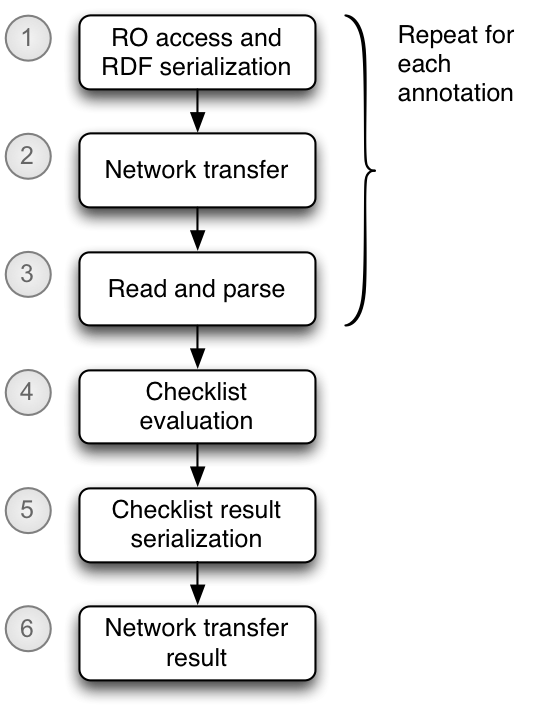
\includegraphics{figures/minim-evaluation-sequence.png}
\caption{Checklist processing model \label{processing}}
\end{figure}

To perform the benchmarking, we created some synthetic ROs with varying
numbers and sizes of annotation files, with aggregate disk usage up to
80Mbytes. The size of the synthesized annotation files was varied by
repeating a group of 11 RDF statements a varying number of times; thus,
an annotation file with 100 annotation groups contains about 1100
separate RDF statements. We also created a trivial checklist whose
actual evaluation time was designed to be minimal on any RO. We used RO
Manager with locally stored ROs to perform the checklist evaluation,
thus avoiding having RO server response and network transfer times
contribute to the results (thereby eliminating contributions to the
recorded running times from steps 1, 2 and 6 in figure
\ref{processing}).

The first tests performed were to confirm that the trivial checklist
evaluation was indeed not taking significant time, by modifying the
checklist evaluation code to short-circuit the actual evaluation logic,
but to perform all other steps. This effectively removed step 4 in
figure \ref{processing}, so the resulting timings would be for steps 3
and 5. Step 5 is assumed to be a small constant time, as the size of the
generated checklist evaluation result depends on the checklist used but
not on the size of the RO (the same trivial checklist was used for all
runs). These timings were compared with an unmodified checklist
evaluation code (performing steps 3, 4 and 5):

Sample timings with checklist evaluation included:

\begin{verbatim}
  Starting evaluation of benchmark_1_10: Mon  7 Oct 2013 16:01:41 BST
               completed benchmark_1_10: Mon  7 Oct 2013 16:01:43 BST
        elapsed time for benchmark_1_10: 2s
  Starting evaluation of benchmark_10_10: Mon  7 Oct 2013 16:01:43 BST
               completed benchmark_10_10: Mon  7 Oct 2013 16:01:44 BST
        elapsed time for benchmark_10_10: 1s
  Starting evaluation of benchmark_100_10: Mon  7 Oct 2013 16:01:44 BST
               completed benchmark_100_10: Mon  7 Oct 2013 16:01:50 BST
        elapsed time for benchmark_100_10: 6s
  Starting evaluation of benchmark_1000_10: Mon  7 Oct 2013 16:01:50 BST
               completed benchmark_1000_10: Mon  7 Oct 2013 16:06:46 BST
        elapsed time for benchmark_1000_10: 296s
  Starting evaluation of benchmark_1_1000: Mon  7 Oct 2013 16:06:46 BST
               completed benchmark_1_1000: Mon  7 Oct 2013 16:06:48 BST
        elapsed time for benchmark_1_1000: 2s
  Starting evaluation of benchmark_10_1000: Mon  7 Oct 2013 16:06:48 BST
               completed benchmark_10_1000: Mon  7 Oct 2013 16:07:10 BST
        elapsed time for benchmark_10_1000: 22s
\end{verbatim}

Sample timings with checklist evaluation excluded:

\begin{verbatim}
  Starting evaluation of benchmark_1_10: Mon  7 Oct 2013 15:53:44 BST
               completed benchmark_1_10: Mon  7 Oct 2013 15:53:45 BST
        elapsed time for benchmark_1_10: 1s
  Starting evaluation of benchmark_10_10: Mon  7 Oct 2013 15:53:45 BST
               completed benchmark_10_10: Mon  7 Oct 2013 15:53:45 BST
        elapsed time for benchmark_10_10: 0s
  Starting evaluation of benchmark_100_10: Mon  7 Oct 2013 15:53:45 BST
               completed benchmark_100_10: Mon  7 Oct 2013 15:53:50 BST
        elapsed time for benchmark_100_10: 5s
  Starting evaluation of benchmark_1000_10: Mon  7 Oct 2013 15:53:50 BST
               completed benchmark_1000_10: Mon  7 Oct 2013 15:58:56 BST
        elapsed time for benchmark_1000_10: 306s
  Starting evaluation of benchmark_1_1000: Mon  7 Oct 2013 15:58:56 BST
               completed benchmark_1_1000: Mon  7 Oct 2013 15:58:57 BST
        elapsed time for benchmark_1_1000: 1s
  Starting evaluation of benchmark_10_1000: Mon  7 Oct 2013 15:58:57 BST
               completed benchmark_10_1000: Mon  7 Oct 2013 15:59:13 BST
        elapsed time for benchmark_10_1000: 16s
\end{verbatim}

(The above figures were obtained running on a MacBook Pro, with a 2.6GHz
Intel Core i7 CPU and 16Gb RAM, using Python 2.7.2 and rdflib 4.01.)

Each benchmark RO used has a name of the form
\texttt{benchmark\_NNN\_SSS}, where \texttt{NNN} is the number of
separate annotation files, and \texttt{SSS} is the size of each file,
measured as a count of ``annotation groups'', where each such group
consists of 11 RDF triples. Thus, \texttt{benchmark\_100\_10} has 100
distinct annotations, each containing 10 annotation groups, or about 110
RDF triples. Each run was performed with freshly-generated ROs, so there
should be no disk cache warming effects between runs.

Some difference between the timings can be seen, but this was generally
within the range of run-to-run variation. The main observation here is
that there is no large and consistent variation between run times with
and without the checklist evaluation step 4 in figure \ref{processing}
included. Accordingly, all remaining benchmarking is performed with the
standard checklist evaluation utility, including the evaluation step,
with a view to understanding how performance varies with size and number
of annotations.

An expanded set of tests was performed to get a picture of how
annotation count and size affect overall checklist evaluation
performance (or, more specifically, the RO annotation load and parse
time). The recorded results of two successive runs are in a spreadsheet
\texttt{Benchmark-summary.xls}\footnote{\url{https://github.com/wf4ever/ro-manager/tree/develop/src/iaeval/benchmark}},
which is in Github along with the benchmark script and supporting code.
For ease of reference, a summary of results is shown in figure
\ref{timings}. We arbitrarily chose 1000 seconds as a cut-off for the
running time of the tests - blank cells in the summary table correspond
to tests which would have taken more than 1000 seconds to complete.

\begin{figure}[htbp]
\centering
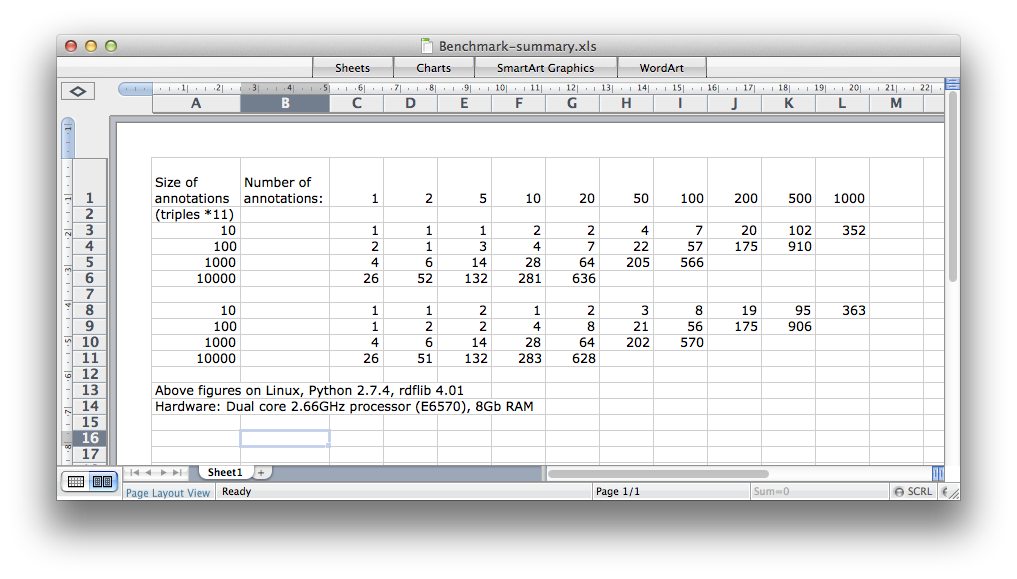
\includegraphics{figures/Benchmark-summary.png}
\caption{Summary of benchmark timings \label{timings}}
\end{figure}

Viewing these as a series of plots of running time vs number of
annotations (figure \ref{time_per_na}), we clearly see that the
performance is super-linear with respect to the number of distinct
annotations.

Viewing these as a series of plots of running time vs size of
annotations (figure \ref{time_per_sa}), it appears that the performance
is linear with respect to the size of the annotations (also borne out by
examination of the numbers).

\begin{figure}[htbp]
\centering
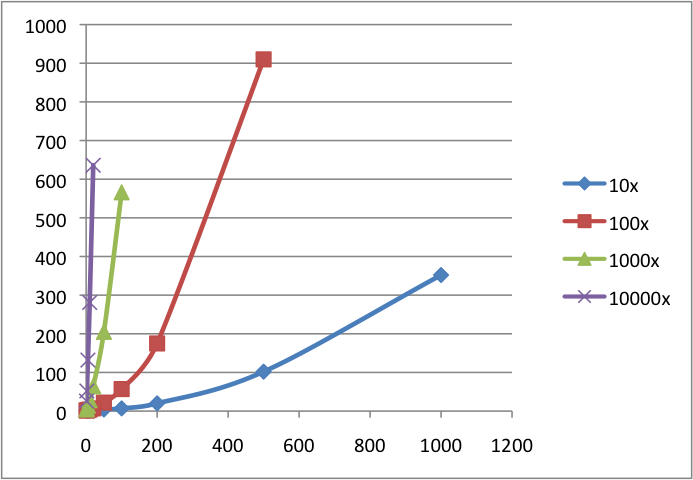
\includegraphics{figures/benchmark-time-per-NA.png}
\caption{Timings vs number of distinct annotation files. (Each trace
corresponds to a particular size of annotation file, indicated as a
count of annotation groups of 11 RDF triples; thus ``100x'' indicates
1100 triples per annotation file.) \label{time_per_na}}
\end{figure}

\begin{figure}[htbp]
\centering
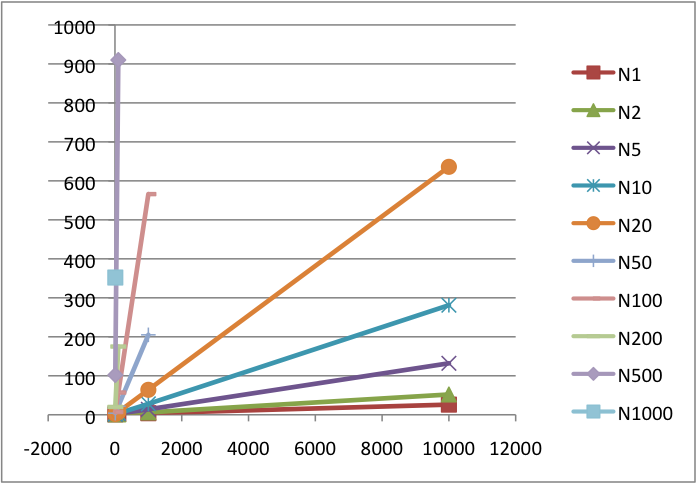
\includegraphics{figures/benchmark-time-per-SA.png}
\caption{Timings vs size of annotations. (Each trace corresponds to an
indicated number of annotation files in the Research Object; thus,
``N20'' indicates 20 distinct annotation files.) \label{time_per_sa}}
\end{figure}

These results support the proposal that the performance bottleneck is
dominated by RDF load and parse times (i.e.~step 3 in figure
\ref{processing}), especially with respect to the number of distinct
annotation resources present. This aspect of performance is almost
entirely dependent on the RDF library and parser used (rdflib\footnote{\url{https://github.com/RDFLib}}).
The choice of library was based upon availability and ease of use with
the chosen programming language environment (Python), and its early
support for SPARQL 1.1 queries. If a different RDF library (and possibly
a different programming language) were to be used, the performance
characteristics are likely to be very different.

\pagebreak [3]

\subsection{Sustainability and maintainability}

The checklist evaluation software has been developed as part of the RO
Manager software suite, and makes use of many of the same components.
This commonality means that fixes developed for one can benefit the
other. The total amount of specific checklist evaluation code\footnote{\url{https://github.com/wf4ever/ro-manager/tree/master/src/iaeval}}
is therefore quite small. The checklist service is built upon the
Pyramid web application framework \footnote{\url{http://docs.pylonsproject.org/projects/pyramid/en/latest/}},
but the amount of dependent code is quite small and porting to the
Django framework \footnote{\url{https://www.djangoproject.com}} has been
considered.

The RO Manager software is packaged and distributed via PyPI \footnote{\url{https://pypi.python.org/pypi/ro-manager}},
and standard Python utilities are used for installation (\texttt{pip},
or \texttt{easy\_install}). These locate and install most external
dependencies. One dependency of the checklist service that is not
automatically installed by the RO Manager package is the Pyramid web
framework, which itself can be installed with all its dependencies by a
single command. Further information about installing and deploying the
checklist service can be found in the checklist service software README
file \footnote{\url{https://github.com/wf4ever/ro-manager/blob/master/src/roweb/README.md}
  (README file for checklist service software)}.

The checklist evaluation software has been designed and developed by a
single programmer, with maintainability and sustainability efforts
focused on technical features (unit and integration tests), and to date
little effort has been committed to developer-community building.

\subsubsection{Survey}

\textbf{Identity:}

To what extent is the identity of the project/software clear and unique
both within its application domain and generally?

\begin{itemize}
\itemsep1pt\parskip0pt\parsep0pt
\item
  Project/software has its own domain name.

  \begin{itemize}
  \itemsep1pt\parskip0pt\parsep0pt
  \item
    No, but it is under the umbrella of the Wf4Ever project
    (\url{http://www.wf4ever-project.org}) which does
  \end{itemize}
\item
  Project/software has a logo.

  \begin{itemize}
  \itemsep1pt\parskip0pt\parsep0pt
  \item
    No, but Wf4Ever project does.
  \end{itemize}
\item
  Project/software has a distinct name within its application area. A
  search by Google on the name plus keywords from the application area
  throws up the project web site in the first page of matches.

  \begin{itemize}
  \itemsep1pt\parskip0pt\parsep0pt
  \item
    Yes (``RO Manager'': 3rd and 9th hits as of 20131001. Adding
    ``wf4ever'' provides only relevant hits on the first page.)
  \end{itemize}
\item
  Project/software has a distinct name regardless of its application
  area. A search by Google on the name plus keywords from the
  application area throws up the project web site in the first page of
  matches.

  \begin{itemize}
  \itemsep1pt\parskip0pt\parsep0pt
  \item
    Yes (``RO Manager'': 3rd and 9th hits as of 20131001. Adding
    ``wf4ever'' provides only relevant hits on the first page.)
  \end{itemize}
\item
  Project/software name does not throw up embarrassing ``did you
  mean\ldots{}'' hits on Google.

  \begin{itemize}
  \itemsep1pt\parskip0pt\parsep0pt
  \item
    OK (Unless ``Did you mean: ROM Manager'' is considered embarassing.)
  \end{itemize}
\item
  Project/software name does not violate an existing trade-mark.

  \begin{itemize}
  \itemsep1pt\parskip0pt\parsep0pt
  \item
    Not obviously
  \end{itemize}
\item
  Project/software name is trade-marked.

  \begin{itemize}
  \itemsep1pt\parskip0pt\parsep0pt
  \item
    No
  \end{itemize}
\end{itemize}

\textbf{Copyright:}

To what extent is it clear who wrote the software and owns its
copyright?

\begin{itemize}
\itemsep1pt\parskip0pt\parsep0pt
\item
  Web site states copyright.

  \begin{itemize}
  \itemsep1pt\parskip0pt\parsep0pt
  \item
    Yes
  \end{itemize}
\item
  Web site states who developed/develops the software, funders etc.

  \begin{itemize}
  \itemsep1pt\parskip0pt\parsep0pt
  \item
    Yes: acknowledgement link to Wf4Ever project front page.
  \end{itemize}
\item
  If there are multiple web sites then these all state exactly the same
  copyright, licencing and authorship.

  \begin{itemize}
  \itemsep1pt\parskip0pt\parsep0pt
  \item
    N/A
  \end{itemize}
\item
  Each source code file has a copyright statement.

  \begin{itemize}
  \itemsep1pt\parskip0pt\parsep0pt
  \item
    Yes
  \end{itemize}
\item
  If supported by the language, each source code file has a copyright
  statement embedded within a constant.

  \begin{itemize}
  \itemsep1pt\parskip0pt\parsep0pt
  \item
    Yes
  \end{itemize}
\end{itemize}

\textbf{Licencing:}

Has an appropriate licence been adopted?

\begin{itemize}
\itemsep1pt\parskip0pt\parsep0pt
\item
  Web site states licence.

  \begin{itemize}
  \itemsep1pt\parskip0pt\parsep0pt
  \item
    Yes
  \end{itemize}
\item
  Software (source and binaries) has a licence.

  \begin{itemize}
  \itemsep1pt\parskip0pt\parsep0pt
  \item
    Yes
  \end{itemize}
\item
  Software has an open source licence.

  \begin{itemize}
  \itemsep1pt\parskip0pt\parsep0pt
  \item
    Yes (MIT)
  \end{itemize}
\item
  Software has an Open Software Initiative (OSI) recognised licence .

  \begin{itemize}
  \itemsep1pt\parskip0pt\parsep0pt
  \item
    Yes (\url{http://opensource.org/licenses/MIT})
  \end{itemize}
\item
  Each source code file has a licence header.

  \begin{itemize}
  \itemsep1pt\parskip0pt\parsep0pt
  \item
    Yes (link to licence description)
  \end{itemize}
\end{itemize}

\textbf{Governance:}

To what extent does the project make its management, or how its software
development is managed, transparent?

\begin{itemize}
\itemsep1pt\parskip0pt\parsep0pt
\item
  Project has defined a governance policy.

  \begin{itemize}
  \itemsep1pt\parskip0pt\parsep0pt
  \item
    No
  \end{itemize}
\item
  Governance policy is publicly available.

  \begin{itemize}
  \itemsep1pt\parskip0pt\parsep0pt
  \item
    N/A
  \end{itemize}
\end{itemize}

\textbf{Community:}

To what extent does/will an active user community exist for this
product?

\begin{itemize}
\itemsep1pt\parskip0pt\parsep0pt
\item
  Web site has statement of number of users/developers/members.

  \begin{itemize}
  \itemsep1pt\parskip0pt\parsep0pt
  \item
    No
  \end{itemize}
\item
  Web site has success stories.

  \begin{itemize}
  \itemsep1pt\parskip0pt\parsep0pt
  \item
    No
  \end{itemize}
\item
  Web site has quotes from satisfied users.

  \begin{itemize}
  \itemsep1pt\parskip0pt\parsep0pt
  \item
    No
  \end{itemize}
\item
  Web site has list of important partners or collaborators.

  \begin{itemize}
  \itemsep1pt\parskip0pt\parsep0pt
  \item
    No (but see Wf4Ever web site)
  \end{itemize}
\item
  Web site has list of the project's publications.

  \begin{itemize}
  \itemsep1pt\parskip0pt\parsep0pt
  \item
    No (but see Wf4Ever web site)
  \end{itemize}
\item
  Web site has list of third-party publications that cite the software.

  \begin{itemize}
  \itemsep1pt\parskip0pt\parsep0pt
  \item
    No
  \end{itemize}
\item
  Web site has list of software that uses/bundles this software.

  \begin{itemize}
  \itemsep1pt\parskip0pt\parsep0pt
  \item
    No
  \end{itemize}
\item
  Users are requested to cite the project if publishing papers based on
  results derived from the software.

  \begin{itemize}
  \itemsep1pt\parskip0pt\parsep0pt
  \item
    No
  \end{itemize}
\item
  Users are required to cite a boilerplate citation if publishing papers
  based on results derived from the software.

  \begin{itemize}
  \itemsep1pt\parskip0pt\parsep0pt
  \item
    No
  \end{itemize}
\item
  Users exist who are not members of the project.

  \begin{itemize}
  \itemsep1pt\parskip0pt\parsep0pt
  \item
    No
  \end{itemize}
\item
  Developers exist who are not members of the project.

  \begin{itemize}
  \itemsep1pt\parskip0pt\parsep0pt
  \item
    No
  \end{itemize}
\end{itemize}

\textbf{Availability:}

To what extent is the software available? (The SSI evaluation guide uses
``accessible'' for this quality, but that has been changed here to avoid
confusion with other uses of ``accessibility'')

\begin{itemize}
\itemsep1pt\parskip0pt\parsep0pt
\item
  Binary distributions are available (whether for free, payment,
  registration).

  \begin{itemize}
  \itemsep1pt\parskip0pt\parsep0pt
  \item
    Yes (PyPI distribution)
  \end{itemize}
\item
  Binary distributions are freely available.

  \begin{itemize}
  \itemsep1pt\parskip0pt\parsep0pt
  \item
    Yes
  \end{itemize}
\item
  Binary distributions are available without the need for any
  registration or authorisation of access by the project.

  \begin{itemize}
  \itemsep1pt\parskip0pt\parsep0pt
  \item
    Yes
  \end{itemize}
\item
  Source distributions are available (whether for free, payment,
  registration).

  \begin{itemize}
  \itemsep1pt\parskip0pt\parsep0pt
  \item
    Yes (PyPI distribution and Github)
  \end{itemize}
\item
  Source distributions are freely available.

  \begin{itemize}
  \itemsep1pt\parskip0pt\parsep0pt
  \item
    Yes
  \end{itemize}
\item
  Source distributions are available without the need for any
  registration or authorisation of access by the project.

  \begin{itemize}
  \itemsep1pt\parskip0pt\parsep0pt
  \item
    Yes
  \end{itemize}
\item
  Access to source code repository is available (whether for free,
  payment, registration).

  \begin{itemize}
  \itemsep1pt\parskip0pt\parsep0pt
  \item
    Yes
  \end{itemize}
\item
  Anonymous read-only access to source code repository.

  \begin{itemize}
  \itemsep1pt\parskip0pt\parsep0pt
  \item
    Yes
  \end{itemize}
\item
  Ability to browse source code repository online.

  \begin{itemize}
  \itemsep1pt\parskip0pt\parsep0pt
  \item
    Yes
  \end{itemize}
\item
  Repository is hosted externally to a single organisation/institution
  in a sustainable third- party repository (e.g.~SourceForge,
  GoogleCode, LaunchPad, GitHub) which will live beyond the lifetime of
  any current funding line.

  \begin{itemize}
  \itemsep1pt\parskip0pt\parsep0pt
  \item
    Yes (\url{https://github.com/wf4ever/ro-manager})
  \end{itemize}
\item
  Downloads page shows evidence of regular releases (e.g.~six monthly,
  bi-weekly, etc.).

  \begin{itemize}
  \itemsep1pt\parskip0pt\parsep0pt
  \item
    Yes, but not to a fixed schedule
    (\url{https://pypi.python.org/pypi/ro-manager}).
  \end{itemize}
\end{itemize}

\textbf{Testability:}

How straightforward is it to test the software to verify modifications?

\begin{itemize}
\itemsep1pt\parskip0pt\parsep0pt
\item
  Project has unit tests.

  \begin{itemize}
  \itemsep1pt\parskip0pt\parsep0pt
  \item
    Yes
  \end{itemize}
\item
  Project has integration tests.

  \begin{itemize}
  \itemsep1pt\parskip0pt\parsep0pt
  \item
    Partial
  \end{itemize}
\item
  For GUIs, project uses automated GUI test frameworks.

  \begin{itemize}
  \itemsep1pt\parskip0pt\parsep0pt
  \item
    N/A
  \end{itemize}
\item
  Project has scripts for testing scenarios that have not been automated
  (e.g.~for testing GUIs).

  \begin{itemize}
  \itemsep1pt\parskip0pt\parsep0pt
  \item
    No
  \end{itemize}
\item
  Project recommends tools to check conformance to coding standards.

  \begin{itemize}
  \itemsep1pt\parskip0pt\parsep0pt
  \item
    No
  \end{itemize}
\item
  Project has automated tests to check conformance to coding standards.

  \begin{itemize}
  \itemsep1pt\parskip0pt\parsep0pt
  \item
    No
  \end{itemize}
\item
  Project recommends tools to check test coverage.

  \begin{itemize}
  \itemsep1pt\parskip0pt\parsep0pt
  \item
    No
  \end{itemize}
\item
  Project has automated tests to check test coverage.

  \begin{itemize}
  \itemsep1pt\parskip0pt\parsep0pt
  \item
    No
  \end{itemize}
\item
  A minimum test coverage level that must be met has been defined.

  \begin{itemize}
  \itemsep1pt\parskip0pt\parsep0pt
  \item
    No
  \end{itemize}
\item
  There is an automated test for this minimum test coverage level.

  \begin{itemize}
  \itemsep1pt\parskip0pt\parsep0pt
  \item
    N/A
  \end{itemize}
\item
  Tests are automatically run nightly.

  \begin{itemize}
  \itemsep1pt\parskip0pt\parsep0pt
  \item
    No
  \end{itemize}
\item
  Continuous integration is supported -- tests are automatically run
  whenever the source code changes.

  \begin{itemize}
  \itemsep1pt\parskip0pt\parsep0pt
  \item
    No
  \end{itemize}
\item
  Test results are visible to all developers/members.

  \begin{itemize}
  \itemsep1pt\parskip0pt\parsep0pt
  \item
    N/A
  \end{itemize}
\item
  Test results are visible publicly.

  \begin{itemize}
  \itemsep1pt\parskip0pt\parsep0pt
  \item
    N/A
  \end{itemize}
\item
  Test results are e-mailed to a mailing list.

  \begin{itemize}
  \itemsep1pt\parskip0pt\parsep0pt
  \item
    N/A
  \end{itemize}
\item
  This e-mailing list can be subscribed to by anyone.

  \begin{itemize}
  \itemsep1pt\parskip0pt\parsep0pt
  \item
    N/A
  \end{itemize}
\item
  Project specifies how to set up external resources e.g.~FTP servers,
  databases for tests.

  \begin{itemize}
  \itemsep1pt\parskip0pt\parsep0pt
  \item
    No (some tests access RODL)
  \end{itemize}
\item
  Tests create their own files, database tables etc.

  \begin{itemize}
  \itemsep1pt\parskip0pt\parsep0pt
  \item
    Many do
  \end{itemize}
\end{itemize}

\textbf{Portability:}

To what extent can the software be used on other platforms?

\begin{itemize}
\itemsep1pt\parskip0pt\parsep0pt
\item
  Application can be built on and run under Windows.

  \begin{itemize}
  \itemsep1pt\parskip0pt\parsep0pt
  \item
    Yes in theory; not tested
  \end{itemize}
\item
  Application can be built on and run under Windows 7.

  \begin{itemize}
  \itemsep1pt\parskip0pt\parsep0pt
  \item
    Yes in theory; not tested
  \end{itemize}
\item
  Application can be built on and run under Windows XP.

  \begin{itemize}
  \itemsep1pt\parskip0pt\parsep0pt
  \item
    Yes in theory; not tested
  \end{itemize}
\item
  Application can be built on and run under Windows Vista.

  \begin{itemize}
  \itemsep1pt\parskip0pt\parsep0pt
  \item
    Yes in theory; not tested
  \end{itemize}
\item
  Application can be built on and run under UNIX/Linux.

  \begin{itemize}
  \itemsep1pt\parskip0pt\parsep0pt
  \item
    Yes
  \end{itemize}
\item
  Application can be built on and run under Solaris.

  \begin{itemize}
  \itemsep1pt\parskip0pt\parsep0pt
  \item
    Not tested
  \end{itemize}
\item
  Application can be built on and run under RedHat.

  \begin{itemize}
  \itemsep1pt\parskip0pt\parsep0pt
  \item
    Yes in theory; not tested
  \end{itemize}
\item
  Application can be built on and run under Debian.

  \begin{itemize}
  \itemsep1pt\parskip0pt\parsep0pt
  \item
    Yes
  \end{itemize}
\item
  Application can be built on and run under Fedora.

  \begin{itemize}
  \itemsep1pt\parskip0pt\parsep0pt
  \item
    Yes in theory; not tested
  \end{itemize}
\item
  Application can be built on and run under Ubuntu.

  \begin{itemize}
  \itemsep1pt\parskip0pt\parsep0pt
  \item
    Yes
  \end{itemize}
\item
  Application can be built on and run under MacOSX.

  \begin{itemize}
  \itemsep1pt\parskip0pt\parsep0pt
  \item
    Yes
  \end{itemize}
\item
  Browser applications run under Internet Explorer.

  \begin{itemize}
  \itemsep1pt\parskip0pt\parsep0pt
  \item
    N/A
  \end{itemize}
\item
  Browser applications run under Mozilla Firefox.

  \begin{itemize}
  \itemsep1pt\parskip0pt\parsep0pt
  \item
    N/A
  \end{itemize}
\item
  Browser applications run under Google Chrome.

  \begin{itemize}
  \itemsep1pt\parskip0pt\parsep0pt
  \item
    N/A
  \end{itemize}
\item
  Browser applications run under Opera.

  \begin{itemize}
  \itemsep1pt\parskip0pt\parsep0pt
  \item
    N/A
  \end{itemize}
\item
  Browser applications run under Safari.

  \begin{itemize}
  \itemsep1pt\parskip0pt\parsep0pt
  \item
    N/A
  \end{itemize}
\end{itemize}

\textbf{Supportability:}

To what extent will the product be supported currently and in the
future?

\begin{itemize}
\itemsep1pt\parskip0pt\parsep0pt
\item
  Web site has page describing how to get support.

  \begin{itemize}
  \itemsep1pt\parskip0pt\parsep0pt
  \item
    No (but common Github tools apply)
  \end{itemize}
\item
  User doc has page describing how to get support.

  \begin{itemize}
  \itemsep1pt\parskip0pt\parsep0pt
  \item
    No
  \end{itemize}
\item
  Software describes how to get support (in a README for command-line
  tools or a Help=\textgreater{}About window in a GUI).

  \begin{itemize}
  \itemsep1pt\parskip0pt\parsep0pt
  \item
    No
  \end{itemize}
\item
  Above pages/windows/files describe, or link to, a description of ``how
  to ask for help'' e.g.~cite version number, send transcript, error
  logs etc.

  \begin{itemize}
  \itemsep1pt\parskip0pt\parsep0pt
  \item
    No
  \end{itemize}
\item
  Project has an e-mail address.

  \begin{itemize}
  \itemsep1pt\parskip0pt\parsep0pt
  \item
    No (but see Wf4ever project)
  \end{itemize}
\item
  Project e-mail address has project domain name.

  \begin{itemize}
  \itemsep1pt\parskip0pt\parsep0pt
  \item
    N/A
  \end{itemize}
\item
  E-mails are read by more than one person.

  \begin{itemize}
  \itemsep1pt\parskip0pt\parsep0pt
  \item
    N/A
  \end{itemize}
\item
  E-mails are archived.

  \begin{itemize}
  \itemsep1pt\parskip0pt\parsep0pt
  \item
    N/A
  \end{itemize}
\item
  E-mail archives are publicly readable.

  \begin{itemize}
  \itemsep1pt\parskip0pt\parsep0pt
  \item
    N/A
  \end{itemize}
\item
  E-mail archives are searchable.

  \begin{itemize}
  \itemsep1pt\parskip0pt\parsep0pt
  \item
    N/A
  \end{itemize}
\item
  Project has a ticketing system.

  \begin{itemize}
  \itemsep1pt\parskip0pt\parsep0pt
  \item
    Yes (Github; also JIRA for Wf4Ever internal use)
  \end{itemize}
\item
  Ticketing system is publicly readable.

  \begin{itemize}
  \itemsep1pt\parskip0pt\parsep0pt
  \item
    Yes
  \end{itemize}
\item
  Ticketing system is searchable.

  \begin{itemize}
  \itemsep1pt\parskip0pt\parsep0pt
  \item
    Yes
  \end{itemize}
\item
  Web site has site map or index.

  \begin{itemize}
  \itemsep1pt\parskip0pt\parsep0pt
  \item
    Yes, via RO Manager page
    \url{https://github.com/wf4ever/ro-manager}, which links to the
    checklist service README file.
  \end{itemize}
\item
  Web site has search facility.

  \begin{itemize}
  \itemsep1pt\parskip0pt\parsep0pt
  \item
    No
  \end{itemize}
\item
  Project resources are hosted externally to a single
  organisation/institution in a sustainbable e-mail archives or
  ticketing system shows that queries are responded to within a week
  (not necessarily fixed, but at least looked at and a decision taken as
  to their priority).

  \begin{itemize}
  \itemsep1pt\parskip0pt\parsep0pt
  \item
    Source code, web pages and developer facilities are hosted in
    GitHub; some supporting material is on Wf4Ever project servers.
  \item
    See also Wf4ever project
  \end{itemize}
\item
  If there is a blog, is it is regularly used.

  \begin{itemize}
  \itemsep1pt\parskip0pt\parsep0pt
  \item
    N/A
  \item
    See also Wf4ever project
  \end{itemize}
\item
  E-mail lists or forums, if present, have regular posts.

  \begin{itemize}
  \itemsep1pt\parskip0pt\parsep0pt
  \item
    N/A
  \end{itemize}
\end{itemize}

\textbf{Analysability:}

How straightforward is it to analyse the software's source release to:
(a) understand its implementation architecture, and (b) understand
individual source code files and how they fit into the implementation
architecture?

\begin{itemize}
\itemsep1pt\parskip0pt\parsep0pt
\item
  Source code is structured into modules or packages.

  \begin{itemize}
  \itemsep1pt\parskip0pt\parsep0pt
  \item
    Yes
  \end{itemize}
\item
  Source code structure relates clearly to the architecture or design.

  \begin{itemize}
  \itemsep1pt\parskip0pt\parsep0pt
  \item
    Yes, but could be improved
  \end{itemize}
\item
  Project files for IDEs are provided.

  \begin{itemize}
  \itemsep1pt\parskip0pt\parsep0pt
  \item
    N/A
  \end{itemize}
\item
  Source code repository is a revision control system.

  \begin{itemize}
  \itemsep1pt\parskip0pt\parsep0pt
  \item
    Yes
  \end{itemize}
\item
  Structure of the source code repository and how this maps to the
  software's components is documented.

  \begin{itemize}
  \itemsep1pt\parskip0pt\parsep0pt
  \item
    Yes. See the README file and linked documents.
  \end{itemize}
\item
  Source releases are snapshots of the repository.

  \begin{itemize}
  \itemsep1pt\parskip0pt\parsep0pt
  \item
    Yes: PyPI releases are created from commits on the repository master
    branch.
  \end{itemize}
\item
  Source code is commented.

  \begin{itemize}
  \itemsep1pt\parskip0pt\parsep0pt
  \item
    Yes
  \end{itemize}
\item
  Source code comments are written in an API document generation mark-up
  language e.g.~JavaDoc or Doxygen.

  \begin{itemize}
  \itemsep1pt\parskip0pt\parsep0pt
  \item
    N/A
  \end{itemize}
\item
  Source code is laid out and indented well.

  \begin{itemize}
  \itemsep1pt\parskip0pt\parsep0pt
  \item
    Yes
  \end{itemize}
\item
  Source code uses sensible class, package and variable names.

  \begin{itemize}
  \itemsep1pt\parskip0pt\parsep0pt
  \item
    Yes, mostly
  \end{itemize}
\item
  There are no old source code files that should be handled by version
  control e.g. ``SomeComponentOld.java''.

  \begin{itemize}
  \itemsep1pt\parskip0pt\parsep0pt
  \item
    Usually not. Some are kept transiently, and removed after changes
    are finalized.
  \end{itemize}
\item
  There is no commented out code.

  \begin{itemize}
  \itemsep1pt\parskip0pt\parsep0pt
  \item
    Some, but generally only kept transiently.
  \end{itemize}
\item
  There are no TODOs in the code.

  \begin{itemize}
  \itemsep1pt\parskip0pt\parsep0pt
  \item
    Lots of TODOs
  \end{itemize}
\item
  Coding standards are required to be observed.

  \begin{itemize}
  \itemsep1pt\parskip0pt\parsep0pt
  \item
    No enforcement
  \end{itemize}
\item
  Project-specific coding standards are consistent with community or
  generic coding standards (e.g.~for C, Java, FORTRAN etc.).

  \begin{itemize}
  \itemsep1pt\parskip0pt\parsep0pt
  \item
    Yes
  \end{itemize}
\end{itemize}

\textbf{Changeability:}

How straightforward is it to modify the software to: (a) address issues,
(b) modify functionality, and (c) add new functionality?

\begin{itemize}
\itemsep1pt\parskip0pt\parsep0pt
\item
  Project has defined a contributions policy.

  \begin{itemize}
  \itemsep1pt\parskip0pt\parsep0pt
  \item
    No
  \end{itemize}
\item
  Contributions policy is publicly available.

  \begin{itemize}
  \itemsep1pt\parskip0pt\parsep0pt
  \item
    No
  \end{itemize}
\item
  Contributors retain copyright/IP of their contributions.

  \begin{itemize}
  \itemsep1pt\parskip0pt\parsep0pt
  \item
    Yes (by default; there is no assignment process).
  \end{itemize}
\item
  Users, user-developers and developers who are not project members can
  contribute.

  \begin{itemize}
  \itemsep1pt\parskip0pt\parsep0pt
  \item
    Yes, through gatekeeper
  \end{itemize}
\item
  Project has defined a stability/deprecation policy for components,
  APIs etc.

  \begin{itemize}
  \itemsep1pt\parskip0pt\parsep0pt
  \item
    No
  \end{itemize}
\item
  Stability/deprecation policy is publicly available.

  \begin{itemize}
  \itemsep1pt\parskip0pt\parsep0pt
  \item
    N/A
  \end{itemize}
\item
  Releases document deprecated components/APIs in that release.

  \begin{itemize}
  \itemsep1pt\parskip0pt\parsep0pt
  \item
    N/A (no components or APIs have been deprecated)
  \end{itemize}
\item
  Releases document removed/changed components/APIs in that release.

  \begin{itemize}
  \itemsep1pt\parskip0pt\parsep0pt
  \item
    N/A (no components or APIs have been removed/changed)
  \end{itemize}
\item
  Changes in the source code repository are e-mailed to a mailing list.

  \begin{itemize}
  \itemsep1pt\parskip0pt\parsep0pt
  \item
    No
  \end{itemize}
\item
  This e-mailing list can be subscribed to by anyone.

  \begin{itemize}
  \itemsep1pt\parskip0pt\parsep0pt
  \item
    N/A
  \end{itemize}
\end{itemize}

\textbf{Evolvability:}

To what extent will the product be developed in the future: (a) for a
future release, and (b) within a roadmap for the product?

\begin{itemize}
\itemsep1pt\parskip0pt\parsep0pt
\item
  Web site describes project roadmap or plans or milestones (either on a
  web page or within a ticketing system).

  \begin{itemize}
  \itemsep1pt\parskip0pt\parsep0pt
  \item
    No
  \end{itemize}
\item
  Web site describes how project is funded/sustained.

  \begin{itemize}
  \itemsep1pt\parskip0pt\parsep0pt
  \item
    No
  \item
    See also Wf4ever project
  \end{itemize}
\item
  We site describes end dates of current funding lines.

  \begin{itemize}
  \itemsep1pt\parskip0pt\parsep0pt
  \item
    No
  \item
    See also Wf4ever project
  \end{itemize}
\end{itemize}

\textbf{Interoperability:}

To what extent does the software's interoperability: (a) meet
appropriate open standards, and (b) function with required and optional
third-party components?

\begin{itemize}
\itemsep1pt\parskip0pt\parsep0pt
\item
  Uses open standards.

  \begin{itemize}
  \itemsep1pt\parskip0pt\parsep0pt
  \item
    Yes (HTTP, RDF, etc.)
  \end{itemize}
\item
  Uses mature, ratified, non-draft open standards.

  \begin{itemize}
  \itemsep1pt\parskip0pt\parsep0pt
  \item
    Yes
  \end{itemize}
\item
  Provides tests demonstrating compliance to open standards.

  \begin{itemize}
  \itemsep1pt\parskip0pt\parsep0pt
  \item
    No
  \end{itemize}
\end{itemize}

\subsection{Summary of evaluation for checklist service}

The checklist evaluation service is targeted at developers who wish to
use the checklist service to provide quality indications of Research
Objects in other components of the Wf4Ever workflow preservation
software, and more generally. Our experiences indicate that the API is
easy to use, and the code base is capable of being understood and
maintained by third party developers.

Checklist creation needs further work to make it accessible to end
users; we have made some initial steps towards this goal \footnote{\url{https://github.com/wf4ever/ro-manager/blob/master/src/checklist/README.md}}
\footnote{\url{https://github.com/wf4ever/ro-manager/blob/master/src/checklist/mkminim.md}}.
The adaptation of checklists by other members of the project team
indicates that existing checklist descriptions are somewhat
understandable and editable by developers with some knowledge of RDF.
SPARQL and the RO Model. The main issue here is for the checklist
designer to have a clear knowledge of the form of RO annotations used by
the ROs to be evaluated (or by the community to whom the checklist is
addressed).

The current checklist service is capable of a fair range of requirements
arising from our own project, and also of those reported in other
quality evaluation work. There are some requirements from other work
that our implementation does not currently support, but many of these
can be addressed by exploiting the extension points in our design to add
new capabilities.

Checklist evaluation performance has been adequate for much of our use
to date, but we have identified potential problems with ROs containg
large annotations, and especially containing large numbers of
annotations. Our benchmarking indicates that the problems are in the
area of RDF load and parse times, which are somewhat determined by the
RDF handing library used. The most problematic aspect in our work has
been the size of provenance traces generated from Taverna workflow runs,
which contain a lot of information that is not used (so far) in any
checklist. We have given some consideration to alternative strategies
for dealing with large RO annotations, but progress on this will be a
topic for future work.

The project has many of the technical requirements for sustainability
and maintainability in place (version control, unit tests, commented
source code, etc.). The main missing technical feature is to use a
continuous integration platform. But it is clear from the SSI checklist
that there are many aspects of developer community building and
communication that are not yet in place. These are points that should be
addressed if a future project attempts to move this service from a
research prototype to a fully fledged software product.

\section{Stability and Reliability service}

\begin{quote}
(Note: in D1.4v2, this component was described as ``Quality evaluation
service'', but here and elsewhere this broader term is used to refer to
a range of services associated with Integrity and Authenticity
evaluation, and this specific component as above.)
\end{quote}

The above introduced completeness of a research object provides
information of the degree by which a research object contains all the
required resources necessary for a purpose (e.g., workflow runnability).
Based on this dimension the stability measures the ability of a workflow
to preserve its overall completeness state throughout a given period of
time. Thereby, stability extends the scope of the analysis from a
particular point in time to a given time period. Parameters like the
impact of the information added or removed from the research object and
of the decay suffered throughout its history are taken into account for
its assessment.

We also have defined during the Y3 of the project another quality
dimension so called reliability which measures the confidence that a
scientist can have in a particular workflow to preserve its capability
to be executed correctly and producing the expected results. A reliable
workflow is expected not only to be free of decay at the moment of being
inspected but also throughout its life. Consequently, in order to
establish the reliability of a workflow we have identified to what
extent it is complete with respect to a number of requirements and how
stable it has been with respect to such requirements historically.

Using these two dimensions we have created an analytic tool (RO
monitoring)\footnote{\url{http://sandbox.wf4ever-project.org/decayMonitoring/visual.html?RO=ro_uri}}
that enables scientists and other stakeholders to visualize these
metrics and have a better understanding of the evolution of workflow
reliability over time. This analytic tool also monitors the current
stored ROs providing a notification service which alerts whenever a RO
suffers of decay.

The formal definition of these dimensions and their scores calculation
can be found at D4.2v2 ``Design, implementation and deployment of
workflow integrity and authenticity maintenance components''
\cite{D4.2v2}, and also at \cite{wf_reliability} \cite{wf_history}.

\subsection{Component description}

The reliability of a workflow measures the ability of a RO for
converging towards a scenario free of decay, i.e.~complete and stable
through time. A reliable workflow is expected not only to be free of
decay at the moment of being inspected but also in general throughout
its life span. Consequently, in order to establish the reliability of a
workflow it becomes necessary to assess to what extent it is complete
with respect to a number of requirements and how stable it has been with
respect to such requirements historically. For that purpose this
component makes used of the different scores for the checklist and
stability assessments and then it calculates the reliability of a RO.

The different scores for the completeness dimension are provided by the
checklist evaluation API\footnote{\url{http://www.wf4ever-project.org/wiki/display/docs/RO+checklist+evaluation+API}}
\footnote{\url{http://www.wf4ever-project.org/wiki/display/docs/Reliability+Evaluation+API}},
and the stability evaluation is subsumed into the reliability API which
provides results for both dimensions simultaneously (see \cite{D4.2v2}
for further details).

\subsection{Usability study}

See also:

\begin{itemize}
\itemsep1pt\parskip0pt\parsep0pt
\item
  Definition of Stability \footnote{\url{http://www.wf4ever-project.org/wiki/display/docs/Definition+of+RO+Stability}}
\item
  Reliability API \footnote{\url{http://www.wf4ever-project.org/wiki/display/docs/Reliability+Evaluation+API}}
\item
  Reliability Notifications \footnote{\url{http://www.wf4ever-project.org/wiki/display/docs/Reliability+Notifications}}
\item
  Visual RO Monitoring \footnote{\url{http://sandbox.wf4ever-project.org/decayMonitoring/visual.html?RO=ro_uri}}
\end{itemize}

\subsubsection{User perspective}

The main usage of the Reliability and Stability services is by using the
RO Monitoring webapp.

To see the monitoring of a RO users have a link in each of the ROs
available in the RO Portal. They will have access to the complete trace
of reliability in an easy visual way. Apart from that, users will be
notified by the notifications system by any variation in terms of
quality of the RO.

Once the RO monitoring tool is opened, a graph containing quality
information over time will be displayed. Users may have the opportunity
to click on specific dates and get the checklist evaluation of that day,
including a description and the possibility to compare it against a
different point in time. As we can see in the following image, the
points in the graph are in three different color (red, yellow, green)
depending on the checklist results.

\begin{figure}[htbp]
\centering
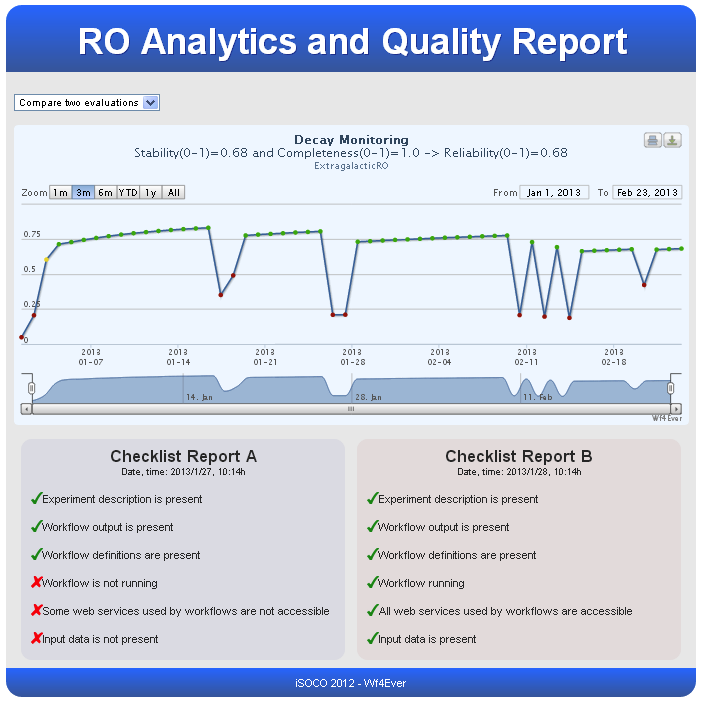
\includegraphics[width=4.7in]{figures/qualityReport2.png}
\caption{RO Analytics and Quality Report}
\end{figure}

The descriptions of the checklist appear under the graph once the user
has clicked on a date. The option to compare two different dates or to
analyze one day only is selected at the Combobox placed on top of the
screen.

\textbf{Survey}

\textbf{General usability:}

\begin{itemize}
\itemsep1pt\parskip0pt\parsep0pt
\item
  Visibility of system status. Does it give users appropriate feedback
  within reasonable time?

  \begin{itemize}
  \itemsep1pt\parskip0pt\parsep0pt
  \item
    Yes. The results appear in a negligible amount of time, providing
    the needed feedback to the user.
  \end{itemize}
\item
  Match between system and the real world. Does it speak the user's
  language and make information appear in a natural and logical order?
  Are implementation-specific details hidden from the user?

  \begin{itemize}
  \itemsep1pt\parskip0pt\parsep0pt
  \item
    Yes. The usage of graphs makes the information understandable. Some
    concepts may require contextual knowledge but are presented in
    user's language.
  \end{itemize}
\item
  User control and freedom. Does it provide clearly marked exits, undo
  and redo?

  \begin{itemize}
  \itemsep1pt\parskip0pt\parsep0pt
  \item
    Yes. The undo and redo are not needed in this application, but
    navigation is very intuitive.
  \end{itemize}
\item
  Consistency and standards. Is it consistent within the software, with
  other similar packages and with platform conventions?

  \begin{itemize}
  \itemsep1pt\parskip0pt\parsep0pt
  \item
    Yes. The languange, interaction with other applications and style
    are aligned with the project standards.
  \end{itemize}
\item
  Error prevention. Does it prevent errors in the first place or help
  users avoid making them?

  \begin{itemize}
  \itemsep1pt\parskip0pt\parsep0pt
  \item
    Yes. The application presents a set of information that doesn't
    allow users make errors. In case something could happen a message
    would appear in order to help users.
  \end{itemize}
\item
  Recognition rather than recall. Does it make objects, actions and
  options visible and reduce the amount of information a user has to
  remember?

  \begin{itemize}
  \itemsep1pt\parskip0pt\parsep0pt
  \item
    Yes. The display and interface is clean and simple.
  \end{itemize}
\item
  Flexibility and efficiency of use. Does it offer short-cuts and
  support macros for frequently- done action sequences?

  \begin{itemize}
  \itemsep1pt\parskip0pt\parsep0pt
  \item
    No. They are not needed.
  \end{itemize}
\item
  Aesthetic and minimalist design. Does it avoid showing irrelevant or
  rarely-needed information?

  \begin{itemize}
  \itemsep1pt\parskip0pt\parsep0pt
  \item
    Yes. Only the needed information is visible.
  \end{itemize}
\item
  Help users recognize, diagnose, and recover from errors. Does it make
  errors clear, comprehensible, precise and suggest solutions if
  possible?

  \begin{itemize}
  \itemsep1pt\parskip0pt\parsep0pt
  \item
    Yes. Errors are clear, but as it is an informative application the
    recoverability is not needed.
  \end{itemize}
\item
  Help and documentation. Does it provide concise, accurate, clear,
  easily-searchable task- oriented doc centred around concrete lists of
  steps?

  \begin{itemize}
  \itemsep1pt\parskip0pt\parsep0pt
  \item
    Yes. There is information on the project main webpage and project
    wiki.
  \end{itemize}
\item
  Robustness. Are responses sensible when instructions are not followed;
  e.g., wrong commands, illegal values, etc.?

  \begin{itemize}
  \itemsep1pt\parskip0pt\parsep0pt
  \item
    Yes. The only possible of error is the retrieval of an inexistent
    Research Object, and a message would appear to inform about that.
  \end{itemize}
\item
  Obviousness. Can tasks be accomplished without any consultation of
  user documents or other material?

  \begin{itemize}
  \itemsep1pt\parskip0pt\parsep0pt
  \item
    Yes. Everything can be used, but a introduction to the concepts
    would be necessary to understand the meaning of the presented
    results.
  \end{itemize}
\end{itemize}

\textbf{Release packaging:}

\begin{itemize}
\itemsep1pt\parskip0pt\parsep0pt
\item
  Are the binary releases packaged for immediate use in a suitable
  archive format?

  \begin{itemize}
  \itemsep1pt\parskip0pt\parsep0pt
  \item
    N/A. Since it is a webservice with a web application, users do not
    need a binary release.
  \end{itemize}
\item
  Is it clear how to get the software from the web site? Does it have
  version numbers?

  \begin{itemize}
  \itemsep1pt\parskip0pt\parsep0pt
  \item
    Yes, in case it is needed there is access to github to download the
    release, but version numbers are not used.
  \end{itemize}
\item
  Is it clear from the web site or user doc what other packages are
  required?

  \begin{itemize}
  \itemsep1pt\parskip0pt\parsep0pt
  \item
    Yes, and they are included in the project.
  \end{itemize}
\item
  Is it clear what the licencing and copyright is on the web site?

  \begin{itemize}
  \itemsep1pt\parskip0pt\parsep0pt
  \item
    Yes, it appears on the site.
  \end{itemize}
\item
  How to get started. Is there a README, FAQ?

  \begin{itemize}
  \itemsep1pt\parskip0pt\parsep0pt
  \item
    Yes, there is information at the project page.
  \end{itemize}
\end{itemize}

\textbf{User documentation:}

\begin{itemize}
\itemsep1pt\parskip0pt\parsep0pt
\item
  Are there relevant user documents?

  \begin{itemize}
  \itemsep1pt\parskip0pt\parsep0pt
  \item
    Yes, there are documents in the project page and wiki. Some of them
    have been provided at the begining of this section.
  \end{itemize}
\item
  Is the user documentation accurate?

  \begin{itemize}
  \itemsep1pt\parskip0pt\parsep0pt
  \item
    Yes, it provides enough information to use the web application.
  \end{itemize}
\item
  Does it partition user, user-developer and developer information or
  mix it all together?

  \begin{itemize}
  \itemsep1pt\parskip0pt\parsep0pt
  \item
    Yes, the information is separated.
  \end{itemize}
\item
  Is the user doc online?

  \begin{itemize}
  \itemsep1pt\parskip0pt\parsep0pt
  \item
    Yes.
  \end{itemize}
\item
  Are there any supporting tutorials?

  \begin{itemize}
  \itemsep1pt\parskip0pt\parsep0pt
  \item
    No, but everything is described in the documentation.
  \end{itemize}
\item
  If so, do these list the versions they apply to?

  \begin{itemize}
  \itemsep1pt\parskip0pt\parsep0pt
  \item
    Not needed.
  \end{itemize}
\item
  If so, are they task-oriented, structured around helping users achieve
  their tasks?

  \begin{itemize}
  \itemsep1pt\parskip0pt\parsep0pt
  \item
    Not needed.
  \end{itemize}
\end{itemize}

\textbf{Help and support:}

\begin{itemize}
\itemsep1pt\parskip0pt\parsep0pt
\item
  Is there a list of known bugs and issues, or a bug/issue tracker?

  \begin{itemize}
  \itemsep1pt\parskip0pt\parsep0pt
  \item
    No. There is no list of bugs.
  \end{itemize}
\item
  Is it clear how to ask for help e.g.~where to e-mail or how to enter
  bugs/issues

  \begin{itemize}
  \itemsep1pt\parskip0pt\parsep0pt
  \item
    Yes. From github one can find the developer's e-mails.
  \end{itemize}
\item
  Are there e-mail list archives or forums?

  \begin{itemize}
  \itemsep1pt\parskip0pt\parsep0pt
  \item
    No.
  \end{itemize}
\item
  If so, is there evidence of use?

  \begin{itemize}
  \itemsep1pt\parskip0pt\parsep0pt
  \item
    Not available.
  \end{itemize}
\item
  Are they searchable?

  \begin{itemize}
  \itemsep1pt\parskip0pt\parsep0pt
  \item
    Not available.
  \end{itemize}
\item
  Is there a bug/issue tracker?

  \begin{itemize}
  \itemsep1pt\parskip0pt\parsep0pt
  \item
    Yes, a private one.
  \end{itemize}
\item
  If so, there evidence of use?

  \begin{itemize}
  \itemsep1pt\parskip0pt\parsep0pt
  \item
    Yes, but not public.
  \end{itemize}
\item
  If so, does it seem that bugs and issues are resolved or, at least,
  looked at?

  \begin{itemize}
  \itemsep1pt\parskip0pt\parsep0pt
  \item
    Depending on the bug.
  \end{itemize}
\item
  Is it clear what quality of service a user expect in terms of support
  e.g.~best effort, reasonable effort, reply in 24 hours etc.?

  \begin{itemize}
  \itemsep1pt\parskip0pt\parsep0pt
  \item
    No, there is no information in respect to that.
  \end{itemize}
\item
  Is it clear how to contribute bugs, issues, corrections (e.g.~in
  tutorials or user doc) or ideas?

  \begin{itemize}
  \itemsep1pt\parskip0pt\parsep0pt
  \item
    There is the possibility of using Github as a generic way.
  \end{itemize}
\end{itemize}

\subsubsection{User-developer perspective}

The user-developers will find that the project is very easy to set up.
Libraries and references are included in the project and as long as
external Research Object and checklist services work, the Stability and
Reliability services will also work. The user-developers will need a
Server to deploy the project and also an Eclipse IDE in case they want
to change part of the functionality and/or customize it.

\textbf{Survey}

\begin{itemize}
\itemsep1pt\parskip0pt\parsep0pt
\item
  How easy is it to set up development environment to write code that
  uses the software or service?

  \begin{itemize}
  \itemsep1pt\parskip0pt\parsep0pt
  \item
    Easy, download the java project (developed in Eclipse IDE) and run
    it on a Tomcat.
  \end{itemize}
\item
  Is it clear what third-party tools and software you need, which
  versions you need, where to get these and how to set them up?

  \begin{itemize}
  \itemsep1pt\parskip0pt\parsep0pt
  \item
    Yes, they are included in the project.
  \end{itemize}
\item
  Are there tutorials available for user-developers?

  \begin{itemize}
  \itemsep1pt\parskip0pt\parsep0pt
  \item
    Not specifically for developers, but the user documents may help.
  \end{itemize}
\item
  If so, Do these list the versions they apply to? Are they accurate,
  and understandable?

  \begin{itemize}
  \itemsep1pt\parskip0pt\parsep0pt
  \item
    Not available.
  \end{itemize}
\item
  Is there example code that can be compiled, customised and used?

  \begin{itemize}
  \itemsep1pt\parskip0pt\parsep0pt
  \item
    The whole project can be compiled and used.
  \end{itemize}
\item
  How accurate, understandable and complete is the API documentation?
  Does it provide examples of use?

  \begin{itemize}
  \itemsep1pt\parskip0pt\parsep0pt
  \item
    Yes, the API is well described and available.
  \end{itemize}
\item
  For services, is there information about quality of service?
  e.g.~number of requests that can be run in a specific time period. How
  do user-developers find out when services might be down etc.

  \begin{itemize}
  \itemsep1pt\parskip0pt\parsep0pt
  \item
    No, this information is not available.
  \end{itemize}
\item
  For services, is there information about copyright and licencing as to
  how the services can be used? e.g.~for non-commercial purposes only,
  does the project have to be credited etc. Is there information on how
  any data can be used, who owns it etc.?

  \begin{itemize}
  \itemsep1pt\parskip0pt\parsep0pt
  \item
    No
  \end{itemize}
\item
  Is the copyright and licencing of the software and third-party
  dependencies clear and documented so you can understand the
  implications on extensions you write?

  \begin{itemize}
  \itemsep1pt\parskip0pt\parsep0pt
  \item
    No
  \end{itemize}
\end{itemize}

\subsubsection{Developer perspective}

The codebase of the application is written in Java, and the API is based
on the use of RESTful web services in the same line of other services
developed for the project. The web applications uses javascript and
jQuery. The code is available at Github and follows the recommended Java
best practices.

Code available at: \url{https://github.com/wf4ever/reliability}

\textbf{Survey}

\begin{itemize}
\itemsep1pt\parskip0pt\parsep0pt
\item
  How easy is it to set up development environment to change the
  software?

  \begin{itemize}
  \itemsep1pt\parskip0pt\parsep0pt
  \item
    It is easy because everything except from the server and eclipse is
    included in the java project.
  \end{itemize}
\item
  How easy is it to access to up-to-date versions of the source code
  that reflect changes made since the last release? i.e.~access to the
  source code repository.

  \begin{itemize}
  \itemsep1pt\parskip0pt\parsep0pt
  \item
    Easy, once they are uploaded to github.
  \end{itemize}
\item
  How easy is it to understand the structure of the source code
  repository? Is there information that relates the structure of the
  source code to the software's architecture?

  \begin{itemize}
  \itemsep1pt\parskip0pt\parsep0pt
  \item
    Medium, it is structured but not described.
  \end{itemize}
\item
  Is it clear what third-party tools and software you need, which
  versions you need, where to get these and how to set them up?

  \begin{itemize}
  \itemsep1pt\parskip0pt\parsep0pt
  \item
    Yes, the information is available in the project.
  \end{itemize}
\item
  How easy is it to compile the code?

  \begin{itemize}
  \itemsep1pt\parskip0pt\parsep0pt
  \item
    Easy, not more difficult than any other code.
  \end{itemize}
\item
  How easy is it to build a release bundle or deploy a service?

  \begin{itemize}
  \itemsep1pt\parskip0pt\parsep0pt
  \item
    Easy, nothing different from a standard service.
  \end{itemize}
\item
  How easy is it to validate changes you've made? This includes building
  the software, getting, building and running tests.

  \begin{itemize}
  \itemsep1pt\parskip0pt\parsep0pt
  \item
    Easy, after the compilation everything can be proved, but there are
    no tests available.
  \end{itemize}
\item
  Is there design documentation available? How accurate and
  understandable is it?

  \begin{itemize}
  \itemsep1pt\parskip0pt\parsep0pt
  \item
    A bit of high level design documentation, but not so much apart from
    commented code and general information at the wiki page.
  \end{itemize}
\item
  Are there tutorials available for developers?

  \begin{itemize}
  \itemsep1pt\parskip0pt\parsep0pt
  \item
    No tutorials for developers.
  \end{itemize}
\item
  If so, are they accurate, and understandable?

  \begin{itemize}
  \itemsep1pt\parskip0pt\parsep0pt
  \item
    Not available.
  \end{itemize}
\item
  How readable is the source code? Well-laid out with good use of
  white-space and indentation?

  \begin{itemize}
  \itemsep1pt\parskip0pt\parsep0pt
  \item
    Readable, indented and with space.
  \end{itemize}
\item
  How accurate or comprehensive is the source code commenting? Does it
  focus on why the code is as it is?

  \begin{itemize}
  \itemsep1pt\parskip0pt\parsep0pt
  \item
    It focuses on adding information for the methods and functions and
    how do they work.
  \end{itemize}
\end{itemize}

\subsection{Benchmarking and performance}

\subsubsection{Capabilities}

The reliability measurement and the implemented visual analytic tool
have the main goal of helping end-users (e.g.~scientist in the
astrophysics and bioinformatics domain) by providing them with a set of
indicators which allow a better judgment of whether they want to use one
RO or another based on how reliable they are. It makes use of the
checklist evaluation service and therefore it also includes the
capabilities that were explained in the section 3.3.1 of this
deliverable. Furthermore it extends these capabilities by adding the
temporal and visual analysis of the structured data provided by the
checklist evaluation service. The main capabilities that are provided
are:

\begin{itemize}
\itemsep1pt\parskip0pt\parsep0pt
\item
  Evaluation and quality assessment of ROs based on the temporal
  information provided by the checklist evaluation service at different
  times.
\item
  Visual temporal detection of workflow decays by using the RO
  monitoring tool. This tool provides a fast glimpse of the historical
  behavior of the RO which have been used and tested by end-users of the
  astronomy domain in order to validate how precise is the decision of
  reusing a RO based on past behavior.
\end{itemize}

These capabilities have been implemented providing a set of new
indicators which have been tested and validated by end users, and by
measuring its usability.

The scenario for validation is the reuse of ROs by scientists. In this
scenario a scientist (Bob) has a list of several tens of galaxies he has
observed during the last years. He is trying to find a workflow that
queries the services of the International Virtual Observatory
(VO)\footnote{\url{http://www.ivoa.net}} in order to gather additional
physical properties for his galaxies. Related to the tag extragalactic,
Bob finds a promising workflow in a research object published by Alice.
He reads its description and finds some similarities to his problem. He
also has a list of galaxies and would like to query several web services
to access their physical properties and perform similar calculations on
them. Bob inspects the research object and, after successfully running
the workflow, finally feels confident that Alice's workflow is a perfect
candidate for reuse in his own work. However, a deeper analysis of its
recent history could prove otherwise:

\begin{enumerate}
\def\labelenumi{\arabic{enumi}.}
\itemsep1pt\parskip0pt\parsep0pt
\item
  The workflow evolution history shows that one of the web services
  changed the format of the input data when adopting ObsTAP VO\footnote{\url{http://www.ivoa.net/Documents/ObsCore}}
  standards for multidata querying. As a consequence the workflow broke,
  and authors had to replace the format of the input dataset.
\item
  This dataset was also used in a script for calculating derived
  properties. The modification of the format of the dataset had
  consequences in the script, which also had to be updated. Bob thinks
  this may be very easily prone to errors.
\item
  Later on, another web service became unavailable during a certain
  time, which turned out that the service provider (in fact Bob's
  research institution) forgot to renew the domain and the service was
  down during two days. The same happened to the input data, since they
  were hosted in the same institution. Bob would prefer now to use his
  own input dataset, and not to rely on these ones.
\item
  This was not the only time the workflow experienced decay due to
  problems with its web services. Recent replacement of networking
  infrastructure (optic fiber and routing hardware) had caused
  connectivity glitches in the same institution, which is the provider
  of the web service and input datasets. Bob needs his workflow working
  regularly, since it continuously looks for upgraded data for his
  statistical study.
\item
  Finally, very recently a data provider modified the output format of
  the responses from HTML to VOTable format in order to be VO compliant
  and achieve data interoperability. This caused one of the scripts to
  fail and required the authors to fix it in order to deal with VOTable
  format instead of proprietary HTML format. Bob thinks this is another
  potential cause for having scripts behaving differently and not
  providing good results.
\end{enumerate}

Even though the workflow currently seems to work well, Bob does not feel
confident about it. The analysis shows that trustworthy reuse by
scientists like Bob depends not only on the degree to which the
properties of a particular workflow and its corresponding research
object are preserved but also on their history. Workflows which can be
executed at a particular point in time might decay and become unrunnable
in the future if they depend on brittle service or data infrastructure,
especially when these belong to third party institutions. Likewise, if
they are subject to frequent changes by their author and contributors,
the probability that some error is introduced also increases.

Due to collecting the necessary data for evaluating the above introduced
scenario using the implemented tools in a real-life setting will require
several years after deployment in a production environment
(e.g.~myExperiment) we have created a scenario which simulates a real
one based on empirical data obtained as result of the study done during
the Y2 of the project {[}3{]}. In that work it was studied the different
types of decay in Taverna workflows and obtained real data about the
distribution of decay during a period of four years. It was also shown
that the most recent workflows are less prone to failures than the older
ones, the main explanation being that workflows seem to be no longer
maintained after some time since their creation. This makes them less
reusable in time, e.g.~the amount of workflows created in 2007 suffering
from decay was 91\% whereas in the case of more recent workflows (2011)
it was around 50\%.

We have used this empirical data for characterizing how workflows decay
along the time and using a sample of 100 workflows during a year we have
identified three main initial groups of workflows: i) G1 contains the
workflow samples which actually run and are well maintained by their
creator or any other user which has a curator role. G1 workflows are
less prone to decay that any other workflow in the other groups; ii) G2
contains those workflows which currently run but are not well maintained
by its creator or by a curator. As a consequence G2 workflows can suffer
from unexpected decay, especially in the event of changes in external
resources necessary for execution; iii) G3 workflows currently do not
work properly and there is no guarantee that they will be curated at
some point.

In order to model the evolution in time of our workflow population we
have considered workflows created over the period from 2007 up to 2011.
We would expect that those created more recently are more likely to be
functioning, while the older workflows are more likely to have decayed.
The distribution of samples considered for each year of creation was
obtained from the study \cite{Zhao-2012}. Table 1 shows the percentage
of decayed workflows, indicating a 41\% decay variation between the
older workflows and those created in 2011. We have used this information
to establish the initial and final states of a decay simulation for
workflows of increasing age: the initial state (S1) contains 50\%
workflows that work correctly (according to the data from 2011) whereas
the final state (S2) contains only 9\% of the workflows that do so
(2007). Using this information we have estimated a distribution of the
number of workflows included in G1, G2 and G3 at the initial and final
states for a total of 100 individuals as G1(S1,S2) = (40, 93),
G2(S1,S2)=(20,0), and G3(S1,S2)=(40, 7).

\begin{longtable}[c]{@{}lrrrrr@{}}
\hline\noalign{\medskip}
Year & 2007 & 2008 & 2009 & 2010 & 2011
\\\noalign{\medskip}
\hline\noalign{\medskip}
Failure \% & 91 & 80 & 90 & 50 & 50
\\\noalign{\medskip}
\hline
\end{longtable}

Table 1: Percentage of workflows suffering decay per year.

Given that the initial state converges towards the final state by a
constant day probability Pd, meaning the likeliness that a workflow
changes to another group, we have defined three parameters: Pd(G1) ∝ (1-
Stability) which establishes the probability that a workflow in G1 (good
health) is downgraded to G3 (bad health), Pd(G2) which follows a random
distribution for establishing the probability that a workflow in G2
shifts to G1 or G3, and Pd(G3) ∝ Stability which establishes the
probability that a workflow in G3 is upgraded to G1. For practical
reasons we have subsumed G2 into G1 and G3 (thus having two groups
representing a bad and good behavior), although preserving its
individual random behavior. Note that decay tends to increase as we
approach the final state S2, hence increasing the population of G3 as
shown in figure \ref{TemporalEvolution} (this shows the explained
evolution of workflows but normalized to one year). The probabilities
that a change occurs in a specific day (Pd) also follow the analysis
results of {[}3{]}. Hereby, we have defined Pd(G1) = 0.49 and Pd(G3) =
0.38, meaning in practice that a workflow will experience three changes
of group on average during the year.

\begin{figure}[htbp]
\centering
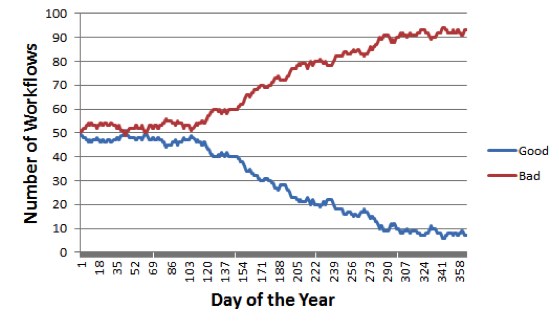
\includegraphics{figures/TemporalEvolution.png}
\caption{Temporal evolution of the two groups (good and bad behavior)
\label{TemporalEvolution}}
\end{figure}

This simulated scenario was implemented following the above explained
model and its pseudocode is shown at figure
\ref{BehaviourEvolutionAlgorithm} where lines 6 and 10 rank the
different workflows of each group proportionally to their stability
values (1 -stability for G3); then lines 7 and 11 take one of them from
the 20\% first ranked workflows. This ranking method reflects the fact
that well maintained workflows will hardly be downgraded from G1 and the
opposite for G3 workflows.

\begin{figure}[htbp]
\centering
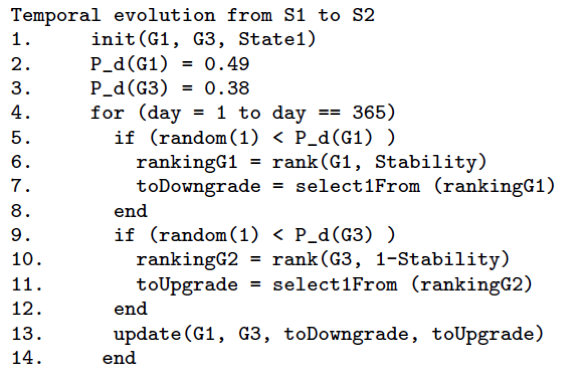
\includegraphics{figures/BehaviourEvolutionAlgorithm.png}
\caption{Algorithm for simulating workflows' behavior evolution
\label{BehaviourEvolutionAlgorithm}}
\end{figure}

The evaluation of the scenario is done by measuring the potential
benefit for a successful reuse taking into account a historical
perspective on the health of scientific workflows, represented by the
reliability score, as opposed to instantaneous quality measures like the
completeness value. To this purpose we run an experiment with nine
scientists (as end users) from the Astrophysics domain\footnote{\url{http://www.iaa.es}}.
At a given point in time, day 274 of the time simulation, we asked them
to look at the completeness values of each of the above mentioned 100
workflows and made them two simple questions:

\begin{enumerate}
\def\labelenumi{\arabic{enumi}.}
\itemsep1pt\parskip0pt\parsep0pt
\item
  Would you reuse this workflow for your own experiments today? and,
\item
  Would you use it in three months from now?
\end{enumerate}

Then, we shuffled the workflows and asked them to answer the questions
again, this time using the RO Monitoring showing the evolution of the
reliability of each workflow until day 274. Then we compare both types
of results with the actual behavior of each workflow today and in three
months. Two of the users did not pass the control test and were
discarded due to the provided answers were outliers. Thus, we focused on
the remaining seven for the evaluation. After applying this criterion we
made a comparative study between using the completeness and reliability
scores, considering the reliability score obtained by the simulation at
the end of the evaluating period, three months ahead, as the ground
truth. Our results showed that 72\% average of the in-the-day reuse
decisions (question 1) obtained better results using the reliability
score, while this value increased to 76\% for question 2. These results
are summarized in Table 2, where ``better choice'' shows the number of
decisions for reusing, taken over specific workflows, which were better
using the provided tool than just using the checklist evaluation service
(the number shown is within the total number of workflows sampled which
was 100). The average improvement distribution for both, question 1 and
2, for each user was 90\%, 85\%, 90\%, 60\%, 75\%, 77\% and 33\%,
respectively. The complete set of results for the both questions can be
seen in tables 3 and 4.

\begin{longtable}[c]{@{}lcc@{}}
\hline\noalign{\medskip}
& Reuse today & Reuse in 3 months
\\\noalign{\medskip}
\hline\noalign{\medskip}
Better choice (\#times) & 51 & 69
\\\noalign{\medskip}
Worse choice (\#times) & 19 & 22
\\\noalign{\medskip}
\hline
\caption{Reliability vs Completeness better choice comparative}
\end{longtable}

Furthermore, the reliability score, and its interpretation through the
RO monitoring tool, allow users to make a better job at managing users'
expectations on the convenience of reusing a workflow today or in three
months. Based on completeness information alone, as shown in Table 5,
whenever we ask users to look ahead one day then 38\% workflows would be
reused, whereas incorporating the reliability information reduces it to
32\% (mainly due to having more information about decay makes users to
be less confident on those ones which failed in the past) and even lower
(28\%) if we ask them to look three months ahead.

\pagebreak [4]

Overall the use of the reliability score improves significantly the
results obtained using completeness information exclusively. In our
experiment we have identified a total of 120 cases where the decision of
what workflows should and should not be reused improved using
reliability values against 41 negative results. This shows evidence that
the use of reliability information, based on the record of workflow
health over time (completeness assessment), enables scientists to make
more informed and better decisions about the reuse of third party
scientific workflows, safeguarding their experiments against decay
potentially introduced by unstable reused workflows.

\begin{longtable}[c]{@{}lcc@{}}
\hline\noalign{\medskip}
& Better choice (\#times) & Worse choice (\#times)
\\\noalign{\medskip}
\hline\noalign{\medskip}
User 1 & 10 & 1
\\\noalign{\medskip}
User 2 & 7 & 1
\\\noalign{\medskip}
User 3 & 9 & 1
\\\noalign{\medskip}
User 4 & 6 & 4
\\\noalign{\medskip}
User 5 & 10 & 4
\\\noalign{\medskip}
User 6 & 6 & 2
\\\noalign{\medskip}
User 7 & 3 & 6
\\\noalign{\medskip}
Total & 51 & 19
\\\noalign{\medskip}
\hline
\caption{Improvement obtained by using reliability score 
instead of using completeness score for today question}
\end{longtable}

\begin{longtable}[c]{@{}lcc@{}}
\hline\noalign{\medskip}
& Better choice (\#times) & Worse choice (\#times)
\\\noalign{\medskip}
\hline\noalign{\medskip}
User 1 & 10 & 1
\\\noalign{\medskip}
User 2 & 10 & 2
\\\noalign{\medskip}
User 3 & 9 & 1
\\\noalign{\medskip}
User 4 & 6 & 4
\\\noalign{\medskip}
User 5 & 19 & 5
\\\noalign{\medskip}
User 6 & 12 & 3
\\\noalign{\medskip}
User 7 & 3 & 6
\\\noalign{\medskip}
Total & 69 & 22
\\\noalign{\medskip}
\hline
\caption{Improvement obtained by using reliability score instead of
using completeness score for from now in 3 months question}
\end{longtable}

\pagebreak [4]

\begin{longtable}[c]{@{}lccc@{}}
\hline\noalign{\medskip}
& Completeness (Today) & Reliability (Today) & Reliability (in 3 months)
\\\noalign{\medskip}
\hline\noalign{\medskip}
User 1 & 42 & 31 & 31
\\\noalign{\medskip}
User 2 & 42 & 34 & 30
\\\noalign{\medskip}
User 3 & 42 & 32 & 32
\\\noalign{\medskip}
User 4 & 20 & 20 & 20
\\\noalign{\medskip}
User 5 & 42 & 32 & 20
\\\noalign{\medskip}
User 6 & 42 & 34 & 27
\\\noalign{\medskip}
User 7 & 42 & 43 & 43
\\\noalign{\medskip}
\hline & & &
\\\noalign{\medskip}
Average & 37.77 $\approx$ 38 & 31.61 $\approx$ 32 & 28.09 $\approx$ 28
\\\noalign{\medskip}
\hline
\caption{Number of times users choose to reuse a workflow based on the
completeness and reliability tools for questions 1 and 2}
\end{longtable}

\subsubsection{Performance}

We have tested the reliability service in order to obtain the maximum
historical data that can be used without having a penalty in the
response to end users which would make the interaction slow. It is known
in the literature\footnote{\url{http://www.stevenseow.com/papers/UI\%20Timing\%20Cheatsheet.pdf}}
that the maximum time of response for instantaneous perception is
$\approx$ 0.1-0.2 secs., and between 0.5-1.0 secs. for immediate
perception which does not need to communicate any indication to the user
to make him aware that the process is ongoing. Considering these values,
we have tested how long backwards, in the historical data of a RO, can
be represented using the developed RO monitoring tool to provide a
instantaneous or immediate perception to end-users (which turns out to
be a response between 0 and 1 sec.). The table 6 shows the results
obtained regarding the time needed to calculate the reliability scores
and response for different number of historical days. If we assume a
maximum time of 1 sec.~as we just mentioned we could provide results
until 2 years and 70 days approximately.

\begin{longtable}[c]{@{}cc@{}}
\hline\noalign{\medskip}
\#Days & Response (msecs.)
\\\noalign{\medskip}
\hline\noalign{\medskip}
1 & 38
\\\noalign{\medskip}
10 & 42
\\\noalign{\medskip}
30 & 48
\\\noalign{\medskip}
182 & 64
\\\noalign{\medskip}
365 (1year) & 105
\\\noalign{\medskip}
730 (2years) & 912
\\\noalign{\medskip}
1095 (3years) & 2355
\\\noalign{\medskip}
\hline
\caption{RO monitoring tool time response for different historical data
periods}
\end{longtable}


\subsection{Sustainability and maintainability}

For short and mid term, the services and web application developed will
be up, available and running. The code will be available for developers
to download it and use it. The way to contact possible future people in
charge of this service is checking the project page or github. There is
not an oficial mailing list for this service but main developers will be
available to answer questions.

\subsubsection{Survey}

\textbf{Identity:}

To what extent is the identity of the project/software clear and unique
both within its application domain and generally?

\begin{itemize}
\itemsep1pt\parskip0pt\parsep0pt
\item
  Project/software has its own domain name.

  \begin{itemize}
  \itemsep1pt\parskip0pt\parsep0pt
  \item
    Yes.
  \end{itemize}
\item
  Project/software has a logo.

  \begin{itemize}
  \itemsep1pt\parskip0pt\parsep0pt
  \item
    No, it uses the project logo.
  \end{itemize}
\item
  Project/software has a distinct name within its application area. A
  search by Google on the name plus keywords from the application area
  throws up the project web site in the first page of matches.

  \begin{itemize}
  \itemsep1pt\parskip0pt\parsep0pt
  \item
    Yes, it appears on google searches using related keywords.
  \end{itemize}
\item
  Project/software has a distinct name regardless of its application
  area. A search by Google on the name plus keywords from the
  application area throws up the project web site in the first page of
  matches.

  \begin{itemize}
  \itemsep1pt\parskip0pt\parsep0pt
  \item
    No, it not appears when using other domain keywords.
  \end{itemize}
\item
  Project/software name does not throw up embarrassing ``did you
  mean\ldots{}'' hits on Google.

  \begin{itemize}
  \itemsep1pt\parskip0pt\parsep0pt
  \item
    No, it is generally correct.
  \end{itemize}
\item
  Project/software name does not violate an existing trade-mark.

  \begin{itemize}
  \itemsep1pt\parskip0pt\parsep0pt
  \item
    No, it does not violate any trade-mark.
  \end{itemize}
\item
  Project/software name is trade-marked.

  \begin{itemize}
  \itemsep1pt\parskip0pt\parsep0pt
  \item
    Yes for the project, not for the specific software.
  \end{itemize}
\end{itemize}

\textbf{Copyright:}

To what extent is it clear who wrote the software and owns its
copyright?

\begin{itemize}
\itemsep1pt\parskip0pt\parsep0pt
\item
  Web site states copyright.

  \begin{itemize}
  \itemsep1pt\parskip0pt\parsep0pt
  \item
    Yes.
  \end{itemize}
\item
  Web site states who developed/develops the software, funders etc.

  \begin{itemize}
  \itemsep1pt\parskip0pt\parsep0pt
  \item
    Yes, links to Wf4ever.
  \end{itemize}
\item
  If there are multiple web sites then these all state exactly the same
  copyright, licencing and authorship.

  \begin{itemize}
  \itemsep1pt\parskip0pt\parsep0pt
  \item
    Not available.
  \end{itemize}
\item
  Each source code file has a copyright statement.

  \begin{itemize}
  \itemsep1pt\parskip0pt\parsep0pt
  \item
    No.
  \end{itemize}
\item
  If supported by the language, each source code file has a copyright
  statement embedded within a constant.

  \begin{itemize}
  \itemsep1pt\parskip0pt\parsep0pt
  \item
    Yes.
  \end{itemize}
\end{itemize}

\textbf{Licencing:}

Has an appropriate licence been adopted?

\begin{itemize}
\itemsep1pt\parskip0pt\parsep0pt
\item
  Web site states licence.

  \begin{itemize}
  \itemsep1pt\parskip0pt\parsep0pt
  \item
    No.
  \end{itemize}
\item
  Software (source and binaries) has a licence.

  \begin{itemize}
  \itemsep1pt\parskip0pt\parsep0pt
  \item
    No
  \end{itemize}
\item
  Software has an open source licence.

  \begin{itemize}
  \itemsep1pt\parskip0pt\parsep0pt
  \item
    Yes (MIT)
  \end{itemize}
\item
  Software has an Open Software Initiative (OSI) recognised licence.

  \begin{itemize}
  \itemsep1pt\parskip0pt\parsep0pt
  \item
    Yes (\url{http://opensource.org/licenses/MIT})
  \end{itemize}
\item
  Each source code file has a licence header.

  \begin{itemize}
  \itemsep1pt\parskip0pt\parsep0pt
  \item
    No.
  \end{itemize}
\end{itemize}

\textbf{Governance:}

To what extent does the project make its management, or how its software
development is managed, transparent?

\begin{itemize}
\itemsep1pt\parskip0pt\parsep0pt
\item
  Project has defined a governance policy.

  \begin{itemize}
  \itemsep1pt\parskip0pt\parsep0pt
  \item
    No.
  \end{itemize}
\item
  Governance policy is publicly available.

  \begin{itemize}
  \itemsep1pt\parskip0pt\parsep0pt
  \item
    Not available.
  \end{itemize}
\end{itemize}

\textbf{Community:}

To what extent does/will an active user community exist for this
product?

\begin{itemize}
\itemsep1pt\parskip0pt\parsep0pt
\item
  Web site has statement of number of users/developers/members.

  \begin{itemize}
  \itemsep1pt\parskip0pt\parsep0pt
  \item
    No.
  \end{itemize}
\item
  Web site has success stories.

  \begin{itemize}
  \itemsep1pt\parskip0pt\parsep0pt
  \item
    No.
  \end{itemize}
\item
  Web site has quotes from satisfied users.

  \begin{itemize}
  \itemsep1pt\parskip0pt\parsep0pt
  \item
    No.
  \end{itemize}
\item
  Web site has list of important partners or collaborators.

  \begin{itemize}
  \itemsep1pt\parskip0pt\parsep0pt
  \item
    No, but they can be seen at Wf4ever page.
  \end{itemize}
\item
  Web site has list of the project's publications.

  \begin{itemize}
  \itemsep1pt\parskip0pt\parsep0pt
  \item
    No, but they can be seen at Wf4ever page.
  \end{itemize}
\item
  Web site has list of third-party publications that cite the software.

  \begin{itemize}
  \itemsep1pt\parskip0pt\parsep0pt
  \item
    No.
  \end{itemize}
\item
  Web site has list of software that uses/bundles this software.

  \begin{itemize}
  \itemsep1pt\parskip0pt\parsep0pt
  \item
    No.
  \end{itemize}
\item
  Users are requested to cite the project if publishing papers based on
  results derived from the software.

  \begin{itemize}
  \itemsep1pt\parskip0pt\parsep0pt
  \item
    No.
  \end{itemize}
\item
  Users are required to cite a boilerplate citation if publishing papers
  based on results derived from the software.

  \begin{itemize}
  \itemsep1pt\parskip0pt\parsep0pt
  \item
    No.
  \end{itemize}
\item
  Users exist who are not members of the project.

  \begin{itemize}
  \itemsep1pt\parskip0pt\parsep0pt
  \item
    Yes, there have been some.
  \end{itemize}
\item
  Developers exist who are not members of the project.

  \begin{itemize}
  \itemsep1pt\parskip0pt\parsep0pt
  \item
    No.
  \end{itemize}
\end{itemize}

\textbf{Availability:}

To what extent is the software available? (The SSI evaluation uses
``accessible'' for this quality, but that has been changed here to avoid
confusion with other uses of ``accessibility'')

\begin{itemize}
\itemsep1pt\parskip0pt\parsep0pt
\item
  Binary distributions are available (whether for free, payment,
  registration).

  \begin{itemize}
  \itemsep1pt\parskip0pt\parsep0pt
  \item
    Not available.
  \end{itemize}
\item
  Binary distributions are freely available.

  \begin{itemize}
  \itemsep1pt\parskip0pt\parsep0pt
  \item
    Not available.
  \end{itemize}
\item
  Binary distributions are available without the need for any
  registration or authorisation of access by the project.

  \begin{itemize}
  \itemsep1pt\parskip0pt\parsep0pt
  \item
    Not available.
  \end{itemize}
\item
  Source distributions are available (whether for free, payment,
  registration).

  \begin{itemize}
  \itemsep1pt\parskip0pt\parsep0pt
  \item
    Yes, on github.
  \end{itemize}
\item
  Source distributions are freely available.

  \begin{itemize}
  \itemsep1pt\parskip0pt\parsep0pt
  \item
    Yes, on github.
  \end{itemize}
\item
  Source distributions are available without the need for any
  registration or authorisation of access by the project.

  \begin{itemize}
  \itemsep1pt\parskip0pt\parsep0pt
  \item
    Yes, no authorization is needed.
  \end{itemize}
\item
  Access to source code repository is available (whether for free,
  payment, registration).

  \begin{itemize}
  \itemsep1pt\parskip0pt\parsep0pt
  \item
    Yes, on github.
  \end{itemize}
\item
  Anonymous read-only access to source code repository.

  \begin{itemize}
  \itemsep1pt\parskip0pt\parsep0pt
  \item
    Yes, on github.
  \end{itemize}
\item
  Ability to browse source code repository online.

  \begin{itemize}
  \itemsep1pt\parskip0pt\parsep0pt
  \item
    Yes, on github.
  \end{itemize}
\item
  Repository is hosted externally to a single organisation/institution
  in a sustainable third- party repository (e.g.~SourceForge,
  GoogleCode, LaunchPad, GitHub) which will live beyond the lifetime of
  any current funding line.

  \begin{itemize}
  \itemsep1pt\parskip0pt\parsep0pt
  \item
    Yes, on github.
  \end{itemize}
\item
  Downloads page shows evidence of regular releases (e.g.~six monthly,
  bi-weekly, etc.).

  \begin{itemize}
  \itemsep1pt\parskip0pt\parsep0pt
  \item
    No.
  \end{itemize}
\end{itemize}

\textbf{Testability:}

How straightforward is it to test the software to verify modifications?

\begin{itemize}
\itemsep1pt\parskip0pt\parsep0pt
\item
  Project has unit tests.

  \begin{itemize}
  \itemsep1pt\parskip0pt\parsep0pt
  \item
    Yes, it has base cases to test it.
  \end{itemize}
\item
  Project has integration tests.

  \begin{itemize}
  \itemsep1pt\parskip0pt\parsep0pt
  \item
    No.
  \end{itemize}
\item
  For GUIs, project uses automated GUI test frameworks.

  \begin{itemize}
  \itemsep1pt\parskip0pt\parsep0pt
  \item
    Not available.
  \end{itemize}
\item
  Project has scripts for testing scenarios that have not been automated
  (e.g.~for testing GUIs).

  \begin{itemize}
  \itemsep1pt\parskip0pt\parsep0pt
  \item
    Not available.
  \end{itemize}
\item
  Project recommends tools to check conformance to coding standards.

  \begin{itemize}
  \itemsep1pt\parskip0pt\parsep0pt
  \item
    Not available.
  \end{itemize}
\item
  Project has automated tests to check conformance to coding standards.

  \begin{itemize}
  \itemsep1pt\parskip0pt\parsep0pt
  \item
    Not available.
  \end{itemize}
\item
  Project recommends tools to check test coverage.

  \begin{itemize}
  \itemsep1pt\parskip0pt\parsep0pt
  \item
    Not available.
  \end{itemize}
\item
  Project has automated tests to check test coverage.

  \begin{itemize}
  \itemsep1pt\parskip0pt\parsep0pt
  \item
    Not available.
  \end{itemize}
\item
  A minimum test coverage level that must be met has been defined.

  \begin{itemize}
  \itemsep1pt\parskip0pt\parsep0pt
  \item
    Not available.
  \end{itemize}
\item
  There is an automated test for this minimum test coverage level.

  \begin{itemize}
  \itemsep1pt\parskip0pt\parsep0pt
  \item
    Not available.
  \end{itemize}
\item
  Tests are automatically run nightly.

  \begin{itemize}
  \itemsep1pt\parskip0pt\parsep0pt
  \item
    Not available.
  \end{itemize}
\item
  Continuous integration is supported -- tests are automatically run
  whenever the source code changes.

  \begin{itemize}
  \itemsep1pt\parskip0pt\parsep0pt
  \item
    Not available.
  \end{itemize}
\item
  Test results are visible to all developers/members.

  \begin{itemize}
  \itemsep1pt\parskip0pt\parsep0pt
  \item
    Not available.
  \end{itemize}
\item
  Test results are visible publicly.

  \begin{itemize}
  \itemsep1pt\parskip0pt\parsep0pt
  \item
    Not available.
  \end{itemize}
\item
  Test results are e-mailed to a mailing list.

  \begin{itemize}
  \itemsep1pt\parskip0pt\parsep0pt
  \item
    Not available.
  \end{itemize}
\item
  This e-mailing list can be subscribed to by anyone.

  \begin{itemize}
  \itemsep1pt\parskip0pt\parsep0pt
  \item
    Not available.
  \end{itemize}
\item
  Project specifies how to set up external resources e.g.~FTP servers,
  databases for tests.

  \begin{itemize}
  \itemsep1pt\parskip0pt\parsep0pt
  \item
    No.
  \end{itemize}
\item
  Tests create their own files, database tables etc.

  \begin{itemize}
  \itemsep1pt\parskip0pt\parsep0pt
  \item
    No.
  \end{itemize}
\end{itemize}

\textbf{Portability:}

To what extent can the software be used on other platforms?

\begin{itemize}
\itemsep1pt\parskip0pt\parsep0pt
\item
  Application can be built on and run under Windows.

  \begin{itemize}
  \itemsep1pt\parskip0pt\parsep0pt
  \item
    Yes.
  \end{itemize}
\item
  Application can be built on and run under Windows 7.

  \begin{itemize}
  \itemsep1pt\parskip0pt\parsep0pt
  \item
    Yes.
  \end{itemize}
\item
  Application can be built on and run under Windows XP.

  \begin{itemize}
  \itemsep1pt\parskip0pt\parsep0pt
  \item
    Yes.
  \end{itemize}
\item
  Application can be built on and run under Windows Vista.

  \begin{itemize}
  \itemsep1pt\parskip0pt\parsep0pt
  \item
    Yes.
  \end{itemize}
\item
  Application can be built on and run under UNIX/Linux.

  \begin{itemize}
  \itemsep1pt\parskip0pt\parsep0pt
  \item
    Yes.
  \end{itemize}
\item
  Application can be built on and run under Solaris.

  \begin{itemize}
  \itemsep1pt\parskip0pt\parsep0pt
  \item
    Not tested.
  \end{itemize}
\item
  Application can be built on and run under RedHat.

  \begin{itemize}
  \itemsep1pt\parskip0pt\parsep0pt
  \item
    Not tested.
  \end{itemize}
\item
  Application can be built on and run under Debian.

  \begin{itemize}
  \itemsep1pt\parskip0pt\parsep0pt
  \item
    Yes.
  \end{itemize}
\item
  Application can be built on and run under Fedora.

  \begin{itemize}
  \itemsep1pt\parskip0pt\parsep0pt
  \item
    Not tested.
  \end{itemize}
\item
  Application can be built on and run under Ubuntu.

  \begin{itemize}
  \itemsep1pt\parskip0pt\parsep0pt
  \item
    Yes.
  \end{itemize}
\item
  Application can be built on and run under MacOSX.

  \begin{itemize}
  \itemsep1pt\parskip0pt\parsep0pt
  \item
    Yes.
  \end{itemize}
\item
  Browser applications run under Internet Explorer.

  \begin{itemize}
  \itemsep1pt\parskip0pt\parsep0pt
  \item
    Yes.
  \end{itemize}
\item
  Browser applications run under Mozilla Firefox.

  \begin{itemize}
  \itemsep1pt\parskip0pt\parsep0pt
  \item
    Yes.
  \end{itemize}
\item
  Browser applications run under Google Chrome.

  \begin{itemize}
  \itemsep1pt\parskip0pt\parsep0pt
  \item
    Yes.
  \end{itemize}
\item
  Browser applications run under Opera.

  \begin{itemize}
  \itemsep1pt\parskip0pt\parsep0pt
  \item
    Not tested.
  \end{itemize}
\item
  Browser applications run under Safari.

  \begin{itemize}
  \itemsep1pt\parskip0pt\parsep0pt
  \item
    Not tested.
  \end{itemize}
\end{itemize}

\textbf{Supportability:}

To what extent will the product be supported currently and in the
future?

\begin{itemize}
\itemsep1pt\parskip0pt\parsep0pt
\item
  Web site has page describing how to get support.

  \begin{itemize}
  \itemsep1pt\parskip0pt\parsep0pt
  \item
    No (but common Github tools apply)
  \end{itemize}
\item
  User doc has page describing how to get support.

  \begin{itemize}
  \itemsep1pt\parskip0pt\parsep0pt
  \item
    No.
  \end{itemize}
\item
  Software describes how to get support (in a README for command-line
  tools or a Help=\textgreater{}About window in a GUI).

  \begin{itemize}
  \itemsep1pt\parskip0pt\parsep0pt
  \item
    No.
  \end{itemize}
\item
  Above pages/windows/files describe, or link to, a description of ``how
  to ask for help'' e.g.~cite version number, send transcript, error
  logs etc.

  \begin{itemize}
  \itemsep1pt\parskip0pt\parsep0pt
  \item
    No.
  \end{itemize}
\item
  Project has an e-mail address.

  \begin{itemize}
  \itemsep1pt\parskip0pt\parsep0pt
  \item
    No, but see Wf4ever project.
  \end{itemize}
\item
  Project e-mail address has project domain name.

  \begin{itemize}
  \itemsep1pt\parskip0pt\parsep0pt
  \item
    Not available.
  \end{itemize}
\item
  E-mails are read by more than one person.

  \begin{itemize}
  \itemsep1pt\parskip0pt\parsep0pt
  \item
    Not available.
  \end{itemize}
\item
  E-mails are archived.

  \begin{itemize}
  \itemsep1pt\parskip0pt\parsep0pt
  \item
    Not available.
  \end{itemize}
\item
  E-mail archives are publicly readable.

  \begin{itemize}
  \itemsep1pt\parskip0pt\parsep0pt
  \item
    Not available.
  \end{itemize}
\item
  E-mail archives are searchable.

  \begin{itemize}
  \itemsep1pt\parskip0pt\parsep0pt
  \item
    Not available.
  \end{itemize}
\item
  Project has a ticketing system.

  \begin{itemize}
  \itemsep1pt\parskip0pt\parsep0pt
  \item
    Yes, github and JIRA.
  \end{itemize}
\item
  Ticketing system is publicly readable.

  \begin{itemize}
  \itemsep1pt\parskip0pt\parsep0pt
  \item
    Only github.
  \end{itemize}
\item
  Ticketing system is searchable.

  \begin{itemize}
  \itemsep1pt\parskip0pt\parsep0pt
  \item
    Yes.
  \end{itemize}
\item
  Web site has site map or index.

  \begin{itemize}
  \itemsep1pt\parskip0pt\parsep0pt
  \item
    No.
  \end{itemize}
\item
  Web site has search facility.

  \begin{itemize}
  \itemsep1pt\parskip0pt\parsep0pt
  \item
    No.
  \end{itemize}
\item
  Project resources are hosted externally to a single
  organisation/institution in a sustainbable e-mail archives or
  ticketing system shows that queries are responded to within a week
  (not necessarily fixed, but at least looked at and a decision taken as
  to their priority).

  \begin{itemize}
  \itemsep1pt\parskip0pt\parsep0pt
  \item
    Some are hosted externally and some are in Wf4ever project servers.
  \end{itemize}
\item
  If there is a blog, is it is regularly used.

  \begin{itemize}
  \itemsep1pt\parskip0pt\parsep0pt
  \item
    Not available.
  \end{itemize}
\item
  E-mail lists or forums, if present, have regular posts.

  \begin{itemize}
  \itemsep1pt\parskip0pt\parsep0pt
  \item
    Not available.
  \end{itemize}
\end{itemize}

\textbf{Analysability:}

How straightforward is it to analyse the software's source release to:
(a) To understand its implementation architecture? (b) To understand
individual source code files and how they fit into the implementation
architecture?

\begin{itemize}
\itemsep1pt\parskip0pt\parsep0pt
\item
  Source code is structured into modules or packages.

  \begin{itemize}
  \itemsep1pt\parskip0pt\parsep0pt
  \item
    Yes.
  \end{itemize}
\item
  Source code structure relates clearly to the architecture or design.

  \begin{itemize}
  \itemsep1pt\parskip0pt\parsep0pt
  \item
    Yes.
  \end{itemize}
\item
  Project files for IDEs are provided.

  \begin{itemize}
  \itemsep1pt\parskip0pt\parsep0pt
  \item
    Yes.
  \end{itemize}
\item
  Source code repository is a revision control system.

  \begin{itemize}
  \itemsep1pt\parskip0pt\parsep0pt
  \item
    Yes.
  \end{itemize}
\item
  Structure of the source code repository and how this maps to the
  software's components is documented.

  \begin{itemize}
  \itemsep1pt\parskip0pt\parsep0pt
  \item
    Part of it.
  \end{itemize}
\item
  Source releases are snapshots of the repository.

  \begin{itemize}
  \itemsep1pt\parskip0pt\parsep0pt
  \item
    Yes.
  \end{itemize}
\item
  Source code is commented.

  \begin{itemize}
  \itemsep1pt\parskip0pt\parsep0pt
  \item
    Yes.
  \end{itemize}
\item
  Source code comments are written in an API document generation mark-up
  language e.g.~JavaDoc or Doxygen.

  \begin{itemize}
  \itemsep1pt\parskip0pt\parsep0pt
  \item
    No.
  \end{itemize}
\item
  Source code is laid out and indented well.

  \begin{itemize}
  \itemsep1pt\parskip0pt\parsep0pt
  \item
    Yes.
  \end{itemize}
\item
  Source code uses sensible class, package and variable names.

  \begin{itemize}
  \itemsep1pt\parskip0pt\parsep0pt
  \item
    Yes.
  \end{itemize}
\item
  There are no old source code files that should be handled by version
  control e.g. ``SomeComponentOld.java''.

  \begin{itemize}
  \itemsep1pt\parskip0pt\parsep0pt
  \item
    There are some that could be needed for other purposes.
  \end{itemize}
\item
  There is no commented out code.

  \begin{itemize}
  \itemsep1pt\parskip0pt\parsep0pt
  \item
    Yes, there is. But could be useful.
  \end{itemize}
\item
  There are no TODOs in the code.

  \begin{itemize}
  \itemsep1pt\parskip0pt\parsep0pt
  \item
    No. There are no TODOs.
  \end{itemize}
\item
  Coding standards are required to be observed.

  \begin{itemize}
  \itemsep1pt\parskip0pt\parsep0pt
  \item
    No.
  \end{itemize}
\item
  Project-specific coding standards are consistent with community or
  generic coding standards (e.g.~for C, Java, FORTRAN etc.).

  \begin{itemize}
  \itemsep1pt\parskip0pt\parsep0pt
  \item
    Yes.
  \end{itemize}
\end{itemize}

\textbf{Changeability:}

How straightforward is it to modify the software to: (a) Address issues?
(b) Modify functionality? (c) Add new functionality?

\begin{itemize}
\itemsep1pt\parskip0pt\parsep0pt
\item
  Project has defined a contributions policy.

  \begin{itemize}
  \itemsep1pt\parskip0pt\parsep0pt
  \item
    No.
  \end{itemize}
\item
  Contributions policy is publicly available.

  \begin{itemize}
  \itemsep1pt\parskip0pt\parsep0pt
  \item
    No.
  \end{itemize}
\item
  Contributors retain copyright/IP of their contributions.

  \begin{itemize}
  \itemsep1pt\parskip0pt\parsep0pt
  \item
    Yes (by default; there is no assignment process).
  \end{itemize}
\item
  Users, user-developers and developers who are not project members can
  contribute.

  \begin{itemize}
  \itemsep1pt\parskip0pt\parsep0pt
  \item
    Yes, contributions are welcome.
  \end{itemize}
\item
  Project has defined a stability/deprecation policy for components,
  APIs etc.

  \begin{itemize}
  \itemsep1pt\parskip0pt\parsep0pt
  \item
    No.
  \end{itemize}
\item
  Stability/deprecation policy is publicly available.

  \begin{itemize}
  \itemsep1pt\parskip0pt\parsep0pt
  \item
    Not available.
  \end{itemize}
\item
  Releases document deprecated components/APIs in that release.

  \begin{itemize}
  \itemsep1pt\parskip0pt\parsep0pt
  \item
    No.
  \end{itemize}
\item
  Releases document removed/changed components/APIs in that release.

  \begin{itemize}
  \itemsep1pt\parskip0pt\parsep0pt
  \item
    No.
  \end{itemize}
\item
  Changes in the source code repository are e-mailed to a mailing list.

  \begin{itemize}
  \itemsep1pt\parskip0pt\parsep0pt
  \item
    No.
  \end{itemize}
\item
  This e-mailing list can be subscribed to by anyone.

  \begin{itemize}
  \itemsep1pt\parskip0pt\parsep0pt
  \item
    Not available.
  \end{itemize}
\end{itemize}

\textbf{Evolvability:}

To what extent will the product be developed in the future: (a) For a
future release? (b) Within a roadmap for the product? 

\begin{itemize}
\itemsep1pt\parskip0pt\parsep0pt
\item
  Web site describes project roadmap or plans or milestones (either on a
  web page or within a ticketing system).

  \begin{itemize}
  \itemsep1pt\parskip0pt\parsep0pt
  \item
    Available at Wf4ever project webpage.
  \end{itemize}
\item
  Web site describes how project is funded/sustained.

  \begin{itemize}
  \itemsep1pt\parskip0pt\parsep0pt
  \item
    Available at Wf4ever project webpage.
  \end{itemize}
\item
  We site describes end dates of current funding lines.

  \begin{itemize}
  \itemsep1pt\parskip0pt\parsep0pt
  \item
    Available at Wf4ever project webpage.
  \end{itemize}
\end{itemize}

\textbf{Interoperability:}

To what extent does the software's interoperability: (a) Meet
appropriate open standards? (b) Function with required third-party
components? (c) Function with optional third-party components?

\begin{itemize}
\itemsep1pt\parskip0pt\parsep0pt
\item
  Uses open standards.

  \begin{itemize}
  \itemsep1pt\parskip0pt\parsep0pt
  \item
    Yes (HTTP, RDF, etc.).
  \end{itemize}
\item
  Uses mature, ratified, non-draft open standards.

  \begin{itemize}
  \itemsep1pt\parskip0pt\parsep0pt
  \item
    Yes.
  \end{itemize}
\item
  Provides tests demonstrating compliance to open standards.

  \begin{itemize}
  \itemsep1pt\parskip0pt\parsep0pt
  \item
    No.
  \end{itemize}
\end{itemize}

\subsection{Summary of evaluation for stability and reliability service}

Scientists, particularly computational scientists, are paying increasing
attention to the methods by which scientific results were obtained.
Amongst the advantages that this offers, it is worthwhile highlighting
some of the following, such as experimental reproducibility and
validation, increased trustworthiness as the basis of subsequent
research, and, more generally speaking, making science more robust,
transparent, pragmatic, and useful.

The implemented stability and reliability service and its RO monitoring
visualization provide a new set of indicators which allow scientist and
other end users to take better decisions regarding when to reuse a
scientific workflow safeguarding their experiments against decay
potentially introduced by unstable reused workflows. This implementation
has been developed following the Wf4Ever project standards and also
trying to accomplish with some characteristics desired by end-users such
as usability (e.g.~providing user documentation, or reasonable response
times), and by developers such as providing releases information, or
code documentation.

To test the complete implementation and some of the usability desired
characteristics we have run some experiments which simulate real
scenarios. These simulations have been based on empirical studies which
have provided the values for creating the models of the experiments. The
results have shown that using these new tool and the calculated
indicators, end-users can take better decision whenever they want to
reuse a scientific experiment.

Furthermore we have tested the usability of the interface (RO monitoring
tool) regarding the amount of time needed to provide a response. This
test has shown that we are currently able to provide a response with an
instantaneous or immediate user perception for around 2 years and 2
months of historical data.

\section{Conclusions}

Scientists, particularly computational scientists, are paying increasing
attention to the methods by which scientific results were obtained.
Amongst the advantages that this offers, it is worth highlighting some
such as experimental reproducibility and validation, increased
trustworthiness as the basis of subsequent research. More generally,
there is a thrust for making science more robust, transparent,
pragmatic, and useful.

The work conducted in WP4 throughout the Wf4Ever project falls within
these lines. In particular our aim has been to contribute to the
conservation and reuse of scientific methods, where reliability plays an
important role. However, reliability cannot be taken simply at face
value. Scientific workflows encoding experimental methods can experience
decay due to different causes. When this happens, the reliability of the
workflow, i.e.~its claimed capability could be seriously undermined by
factors that are not immediately apparent. Our approach aims at
providing a more complete picture of the changes that may occur to a
workflow over a time period in order to assist scientists in
establishing a more truthful indication of its reliability.

In this deliverable, we evaluate the work of WP4 and particularly the
tools implementing it, which were presented in previous deliverables
D4.1 and D4.2, respectively. Results published elsewhere
\cite{wf_history} prove that the minimal set of information that we
identified as necessary to be associated within a research object can
enable us to assess specific quality metrics of a workflow at a time
point and to monitor the change of this quality measures over a time
period. In this particular deliverable we extend such work with an
evaluation focused on the software components implementing such
functionalities. To this purpose, we have assessed the performance of
the two main tools created to proactively evaluate and monitor the
health of Research Objects, namely the checklist service and the
stability and reliability service.

The evaluation presented herein is structured around the guidelines
provided by the UK's Software Sustainability Institute (SSI) for
Software evaluation guide. Following the guidelines, we have targeted
three kinds of user: end-users, i.e., non-developers who will employ the
software, developer-users, i.e., developers who will use APIs and other
middleware facilities provided in the creation of some wider
application, and developers, i.e., those tasked with enhancing or
repairing the software. The results obtained show evidence of the
usefulness of the components for the different types of users and of
promising software sustainability after the end of the project.

We believe our work can have a strong impact in the incremental
development of scientific knowledge, especially in those disciplines
related to in-silico experimentation, where the reuse of existing work
is paramount. New publication paradigms involving semantic publications
can benefit from our approach, supporting the development and
publication of new scientific advances based on the reuse of
reproducible and reliable previous work. To this purpose, we are
collaborating with publishers like
Gigascience\textasciitilde{}\footnote{http://www.gigasciencejournal.com}
and the American Psychological
Association\textasciitilde{}\footnote{http://www.apa.org} (APA) as well
as with scientific digital libraries like NASA's
ADS\textasciitilde{}\footnote{http://adswww.harvard.edu} interested in
the application of our methods and tools.
